\documentclass[review]{elsarticle}

%% Necessary packages
\usepackage{graphicx}   
\usepackage{amssymb}    
\usepackage{amsmath}  
\usepackage{xcolor}     
\usepackage{graphicx}   
\usepackage{subcaption} 
\usepackage{placeins} 
\usepackage{float}    
\usepackage{soul}
\usepackage{verbatim}
\usepackage{graphicx}
\usepackage{subcaption}
\usepackage[a4paper, margin=1in]{geometry}
\usepackage[colorlinks=true, linkcolor=black, citecolor=black, urlcolor=blue]{hyperref}

%% --- Reviewer suggestion markup (SJL) ---
\definecolor{sjlmutedred}{RGB}{180, 80, 80}
\definecolor{sjlmutedblue}{RGB}{70, 100, 180}
\DeclareRobustCommand{\suggestreplacesjl}[2]{%
  {\color{sjlmutedred}\textbf{[SJL20260305, Suggested Text to be Replaced]}\ #1}%
  \ {\color{sjlmutedblue}\textbf{[SJL20260305, Suggested New Text]}\ #2}%
}




%% Journal name
\journal{Applied Energy}

\begin{document}

\begin{frontmatter}

%% Title
\title{Electricity Access Is Not Enough: Evidence from Voltage Quality Monitoring in Kampala’s Informal Settlements}

%% Authors and affiliations

\author[inst1]{Civian Kiki Massa\corref{cor1}}
\ead{ckmassa@umass.edu}
\author[inst2]{Jessica Kersey}
\author[inst3]{Paul Kyoma Asiimwe}
\author[inst4]{Margaret Odero}
\author[inst5]{June Lukuyu}
\author[inst6]{Stephen Lee}
\author[inst7]{Judith Mbabazi}
\author[inst8]{Laura Kwong}
\author[inst9]{Jay Taneja}

\cortext[cor1]{Corresponding author}

%% Affiliations

\affiliation[inst1]{organization={Department of Electrical and Computer Engineering},
            addressline={University of Massachusetts Amherst},
            city={Amherst},
            state={MA},
            country={USA}}

\affiliation[inst2]{organization={Energy and Resources Group},
            addressline={University of California, Berkeley},
            city={Berkeley},
            state={CA},
            country={USA}}

\affiliation[inst3]{organization={Department of Electrical and Electronics Engineering},
            addressline={Makerere University},
            city={Kampala},
            country={Uganda}}

\affiliation[inst4]{organization={nLine.Inc},
            city={},
            country={USA}}

\affiliation[inst5]{organization={Department of Electrical and Computer Engineering},
            addressline={University of Washington},
            city={Seattle},
            state={WA},
            country={USA}}

\affiliation[inst6]{organization={Manning College of Information and Computer Sciences},
            addressline={University of Massachusetts Amherst},
            city={Amherst},
            state={MA},
            country={USA}}

\affiliation[inst7]{organization={Geography, Geo-informatics and Climatic Sciences},
            addressline={Makerere University},
            city={Kampala},
            country={Uganda}}

\affiliation[inst8]{organization={Division of Environmental Health Sciences},
            addressline={University of California, Berkeley},
            city={Berkeley},
            state={CA},
            country={USA}}

\affiliation[inst9]{organization={Manning College of Information and Computer Sciences},
            addressline={University of Massachusetts Amherst},
            city={Amherst},
            state={MA},
            country={USA}}



%% Abstract
\begin{abstract}
A grid connection alone does not ensure safe, usable, or equitable electricity access, particularly in rapidly urbanizing informal settlements. This study presents a high-resolution analysis of voltage quality across 25 formal and informal communities in Kampala, Uganda. We deployed voltage quality sensors in 150 households and businesses (100 in informal and 50 in nearby formal areas) and conducted surveys and wiring inspections in the same communities. While 95\% of households in informal areas are technically grid-connected, over 20\% of voltage samples fall below acceptable thresholds, with undervoltage lasting an average of 6.3 hours per day-nearly triple that of formal areas. Unmetered users face significantly poorer voltage quality, often relying on informal wiring due to high connection fees and bureaucratic challenges. To assess how stable or chaotic voltage conditions are over time, we apply \suggestreplacesjl{an entropy matrix and a semi-Markov state-transition analysis}{entropy-based predictability measures and a first-order Markov state-transition analysis over a duration-enriched state space}. Our results show that voltage quality in informal areas is not only poor, but also temporally volatile, especially during peak demand periods. Field inspections reveal unmetered connections, unsafe wiring and exposed connections as common contributors to these issues. These findings show that electricity access in such contexts is shaped not only by grid supply, but also by connection modalities and behind-the-meter infrastructure. We argue that definitions of “modern energy access” must expand to include power quality, temporal predictability, and infrastructural safety-dimensions that directly affect usability, appliance performance, and the feasibility of energy transitions such as electric cooking and other energy services.

\end{abstract}

%% Highlights
\begin{highlights}
\item Power quality sensors were deployed to monitor voltage quality and reliability in 25 urban informal and formal settlements for over 2 months
\item Informal settlements experience prolonged low voltage conditions and severe voltage variations compared to formal settlements
\item Connection modalities significantly influence poor voltage conditions,  with unmetered users facing the most unreliable power supply.
\item \suggestreplacesjl{Predictability of voltage fluctuations and low voltage events are demonstrated with a 3-dimensional state transition probability and entropy model}{Predictability of voltage fluctuations and low voltage events is characterized using a Markov chain voltage quality model with entropy-based predictability measures}
\item Results challenge binary access metrics and highlight voltage quality, connection modalities and  “temporal energy poverty”
\end{highlights}



%% Keywords
\begin{keyword}
Voltage quality \sep urban informal settlements \sep energy access \sep connection modalities 
\end{keyword}

\end{frontmatter}

%% Main text
\section{Introduction}
\label{sec:intro}
Access to reliable, usable and affordable electricity is foundational to economic development and social well-being. Globally, significant progress has been made toward Sustainable Development Goal 7 (SDG7), which aims to ensure universal access to affordable, reliable, sustainable, and modern energy. The number of people without electricity dropped from 1.2 billion in 2010 to approximately 600 million in 2023 \cite{SDG7Report2020, IEA2023Electricity, ayaburi2020measuring}. However, this progress has been uneven. Much of the improvement has occurred in South and Southeast Asia, where countries like Vietnam, Bangladesh, and India have seen near-universal electrification, while Sub-Saharan Africa (SSA) remains home to over 85\% of the global population still lacking access \cite{sdg72025, IEA2024SDG7}.

At the same time, rapid urbanization is reshaping the energy landscape. By 2050, 70\% of the global population is expected to live in urban areas \cite{broto2017energy, adams2018intra}, with the fastest growth 
occurring in cities across the Global South. In Africa, approximately 60\% of the urban population resides in informal settlements—also known as slums—which are often characterized by insecure tenure, inadequate infrastructure, and limited access to public services, including electricity \cite{Cabrita2024Preprint, Madzivhandila2024Climate, TodesGoodfellow2024, adams2017water}. 


In these dense and underserved areas, electrification is not only incomplete but also qualitatively deficient. While binary access indicators (connected vs. unconnected) suggest urban electrification rates above 80\% in SSA, many connected households experience poor power quality, frequent outages, and unsafe wiring conditions. These limitations significantly reduce the usability of electricity for essential services such as cooking, refrigeration, lighting, healthcare, and small business operations \cite{stevanato2023access, mensah2022electricity}. 

Electricity access has historically been measured using binary indicators that classify households as  connected or unconnected, a simplification that masks substantial variation in service quality and usability \cite{WorldBankESMAP2018, IEA2023Electricity}. Recognizing these limitations, the World Bank introduced the Multi-Tier Framework (MTF), which conceptualizes electricity access as a multidimensional continuum encompassing capacity, availability, reliability, quality, affordability, legality, and safety \cite{BhatiaAngelou2015}. However, in practice, MTF implementation relies largely on survey-based instruments and threshold compliance criteria, with voltage quality typically assessed through nominal range checks or self-reported appliance functionality. While these measures capture whether minimum standards are met, they offer limited insight into the temporal dynamics of supply, particularly the persistence, volatility, and predictability of voltage conditions at the point of connection. As a result, systems that formally satisfy tier requirements may still exhibit prolonged undervoltage events, high intra-day variability, or distribution-level instability that constrain productive electricity use. In dense informal settlements, such systems may effectively function as low-capacity lighting and phone-charging platforms rather than as stable infrastructures capable of supporting electric cooking, refrigeration, healthcare delivery, or small enterprise activity. Addressing this gap requires moving beyond static tier classification toward high-frequency empirical measurement of voltage behavior and its temporal structure, an objective that motivates the present study.

\begin{comment}
    Existing energy access frameworks often overlook the dimension of power quality—particularly voltage consistency, predictability, and safety—which is critical for a just and functional energy transition. In informal settlements, poor power quality is not solely a result of appliance inefficiency but is also influenced by multiple contributing factors, including inadequate grid infrastructure, substandard wiring, and diverse, often informal connection modalities \cite{yaguma2023asset, monyai2023inequality}. Despite this, voltage quality and its predictability at the household and small business level remain largely unmeasured and unaddressed in policy and utility planning.
\end{comment}

This paper addresses these knowledge gaps through a unique empirical study of power quality across informal and formal communities in Kampala, Uganda. We argue that a multidimensional access framework is needed to meaningfully characterize electricity access in informal settlements, one that incorporates not just connection status, but voltage quality, predictability, and infrastructure safety. We present one of the most detailed, high-frequency, and longitudinal voltage quality datasets collected from urban informal settlement households and businesses in Kampala, Uganda. Through this dataset, the study provides a rare direct comparison of voltage quality and metering conditions across formal and informal settlements, revealing spatial and infrastructural disparities. It introduces a novel analytical framework that applies \suggestreplacesjl{an entropy matrix and semi-Markov transition modeling}{entropy-based predictability measures and Markov transition modeling over a duration-enriched state space} to characterize the temporal predictability and volatility of voltage conditions—an important but underexplored dimension of electricity access. We also integrate sensor data with infrastructure audits, household surveys, and interviews, to offer a multidimensional perspective on the lived experience of voltage quality. Furthermore, it identifies how socioeconomic status, metering status, and connection modalities interact to shape electricity reliability and quality, offering new insights into distribution-level inequities. Finally, the study highlights power quality as a critical yet overlooked barrier to inclusive electrification and a just energy transition—particularly in contexts where electric cooking, small business activity, and basic service delivery depend on stable and usable electricity.


%Although many studies and practical applications focus on identifying customer equipment as the cause of power quality issues, the scenario in low-income urban settings, particularly informal settlements, presents a more complex situation [cite, source]. These settings are very low consumers of electricity (electricity is mainly used for lighting and other basic needs)  yet they experience some of the worst power quality and reliability issues [source]. This implies that there are other factors beyond inefficient appliances influencing power quality in these settings. Most of their wiring materials are of poor quality, the connection modalities are diverse, and the overall quality of the wiring of most homes and businesses is subpar. These characteristics of the endpoint distribution infrastructure affect the quality of the voltage in complex ways. Furthermore, overloaded transformers and inadequate maintenance of the network providers' infrastructure also contribute to the poor quality of power experienced by consumers in these settings [cite]. 


\section{Background}
\label{sec:Back}
Power quality (PQ) is a multidimensional concept that lacks a universally agreed-upon definition and is often used interchangeably with supply reliability, service quality, voltage quality, or quality of supply \cite{Bollen2000, Dugan2012} In general, power quality refers to the degree to which voltage, current, frequency, and waveform characteristics conform to established technical standards required for the safe and efficient operation of electrical equipment \cite{IEEE1159_2019}. The Institute of Electrical and Electronics Engineers (IEEE) defines power quality as “the concept of powering and grounding sensitive equipment in a manner that is suitable to the operation of that equipment” \cite{IEEE1100_2005}. Similarly, the International Electrotechnical Commission (IEC 61000-4-30) defines it as the “characteristics of the electricity at a given point on an electrical system, evaluated against a set of reference technical parameters” \cite{IEC61508_2010_CMV}. These definitions emphasize that PQ is evaluated relative to technical limits governing voltage magnitude, frequency stability, waveform integrity, and grounding conditions.
 
Power quality phenomena are typically grouped into normal variations and sudden events \cite{Bollen2003}. Normal variations refer to small changes in voltage, frequency, or waveform that occur during everyday operation of the power system. Sudden events involve larger and more noticeable changes from normal conditions and can lead to equipment malfunction or temporary loss of power. Common disturbances include voltage interruptions, undervoltages and overvoltages, transients, voltage unbalance, waveform distortion (such as harmonics and interharmonics), voltage fluctuations (flicker), and frequency variations \cite{Dugan2012, Arrillaga2000}. Given the multidimensional nature of PQ, this study focuses specifically on the voltage quality dimension of power quality, examining sustained deviations in voltage magnitude rather than current distortion, harmonic content, or frequency variation.

\subsection{Sustained voltage deviations }
When voltage deviations persist for over 1 minute, they are considered sustained or long-duration voltage variations. These long-duration variations can be categorized as overvoltage, undervoltage, or sustained interruptions. An overvoltage occurs when the RMS AC voltage rises above 110\% of the nominal voltage at power frequency for more than 1 minute, while an undervoltage occurs when the RMS voltage drops to 90\% of the nominal voltage at power frequency for more than 1 minute. A sustained interruption (outage) happens when the voltage drops to 0 for over 1 minute \cite{Caramia2009}. It's important to note that different countries have varying tolerance limits for these voltage changes, set by their energy regulatory bodies based on local preferences, demand uncertainties, infrastructure quality, technological advancements, safety standards, and economic considerations \cite{IEEE1159_2019, ANSI_C84_1_2020, PowerSonicVoltageCountry}. In Uganda, the tolerance level for overvoltage is set at 106\% and 94\% for undervoltage. In the United States, household electrical outlets have tolerance levels of 105\% for undervoltage and 95\% for overvoltage \cite{UgandaGridCode2003, UgandaBuildingCode2019, ANSI_C84_1_2020}. Although specific tolerance bands vary by jurisdiction, such standards establish the operational boundaries within which electrical equipment is expected to function safely and efficiently.

\subsection{Structural Drivers of Sustained Voltage Deviations at the Point of Connection }

This study evaluates voltage quality at the point of connection, where households experience electricity supply conditions. Although voltage deviations originate from broader distribution network dynamics, the magnitude and persistence of these deviations are shaped not only by feeder-level constraints but also by service-line characteristics, and local wiring configurations(\textbf{source})

In many low-voltage radial distribution systems, voltage magnitude decreases along the feeder due to line resistance and reactance. When current flow increases, particularly during peak demand period, the resulting voltage drop across feeder impedance can produce sustained undervoltage at downstream nodes (\textbf{source}). However, the voltage ultimately experienced within a household also depends on the electrical path between the transformer and the point of connection.

Service-line length, conductor cross-sectional area, and joint quality influence the effective impedance between the transformer secondary and the customer endpoint. Long service drops, undersized conductors, loose terminals, or corroded connections increase resistive losses, resulting in additional voltage reduction under load (\textbf{source}). In densely populated or informally developed areas, these effects are often amplified by shared meters, extended branching from a single service drop, and improvised wiring extensions. Such configurations increase aggregate loading on conductors that were not designed for multi-household demand, thereby magnifying voltage sensitivity to load fluctuations.



\begin{comment}
    It is important for the voltage at endpoints to comply with all standards of the national grid code to ensure the efficient functioning of electric appliances. Customers are responsible for purchasing and using compatible appliances to draw currents without injecting or drawing polluting currents (non-sinusoidal currents) from the network. When appliances operate under voltage conditions below their intended specifications, they may attempt to draw current beyond their design limits to meet their power needs. This can result in decreased efficiency, motor malfunctions, and damage to electronic components. While instances of high-voltage events are less frequent than low-voltage events in low-income communities, they can also pose risks by causing insulation breakdowns and premature failure of equipment. 

    [Source] surveyed 2001 grid-connected households and businesses in Accra, Ghana, and 26\% reported damaged appliances resulting from poor power quality in the past month. Enterprises that participated in another study conducted by [source] in Tanzania also attributed appliance damage to voltage fluctuations and poor power quality. 30\% of participants in our wiring inspections and infrastructure assessment study had appliances damaged while in use or plugged in in the past month. Percolators, fridges, protective devices, TVs, sockets, and electric lamps represent over 70\% of the damaged appliances. Renters reported more broken appliances than homeowners. 
\end{comment}



\subsection{Wiring quality and connection configurations }
Connection modality further shapes the structure of last-mile electricity distribution. In many informal settlements of Sub-Saharan Africa, households access electricity through a range of configurations that differ from standard utility-installed service arrangements. These practices often emerge in response to high connection costs, tariff affordability constraints, and insecure land tenure, particularly among renters.

Although numerous wiring arrangements were observed, three primary connection modalities were prevalent in the study communities: (i) a regular metered connection, (ii) a meter-bypass configuration, and (iii) a direct tap connection as shown in  Figure~\ref{fig:grid_configs}

A regular metered connection follows the standard utility service configuration. Electricity is delivered from the distribution transformer to an individual dwelling through a dedicated service drop terminating at a utility-installed meter. Downstream of the meter, internal wiring distributes electricity to circuits within a single dwelling. Billing is based on recorded consumption at the meter, and the installation typically conforms to utility-approved conductor sizing, protective devices, and grounding practices. The electrical topology in this case reflects a one-to-one relationship between service point and dwelling.
In a meter-bypass configuration, electricity is drawn upstream of the registered meter or routed around it. Although a meter may be physically present, some or all of the load is supplied through conductors that do not pass through the metering device. Electrical distribution within the dwelling or cluster of dwellings may resemble that of a regular connection, but energy consumption is not fully captured by the utility’s metering system. From a network topology perspective, the service connection remains tied to the formal low-voltage feeder, but metering and load accounting are partially circumvented.
A direct tap involves drawing electricity directly from a low-voltage conductor or service line without a utility-installed meter at the point of use. The connection may be made at the feeder, service drop, or transformer secondary conductors. Electricity is then redistributed through locally installed wiring networks that function as informal sub-distribution systems. In this configuration, there is no dedicated metered service point for the dwelling, and internal distribution is organized through branching conductors supplying one or multiple users.

\begin{figure}[!ht]
    \centering

    \begin{subfigure}[b]{0.32\textwidth}
        \centering
        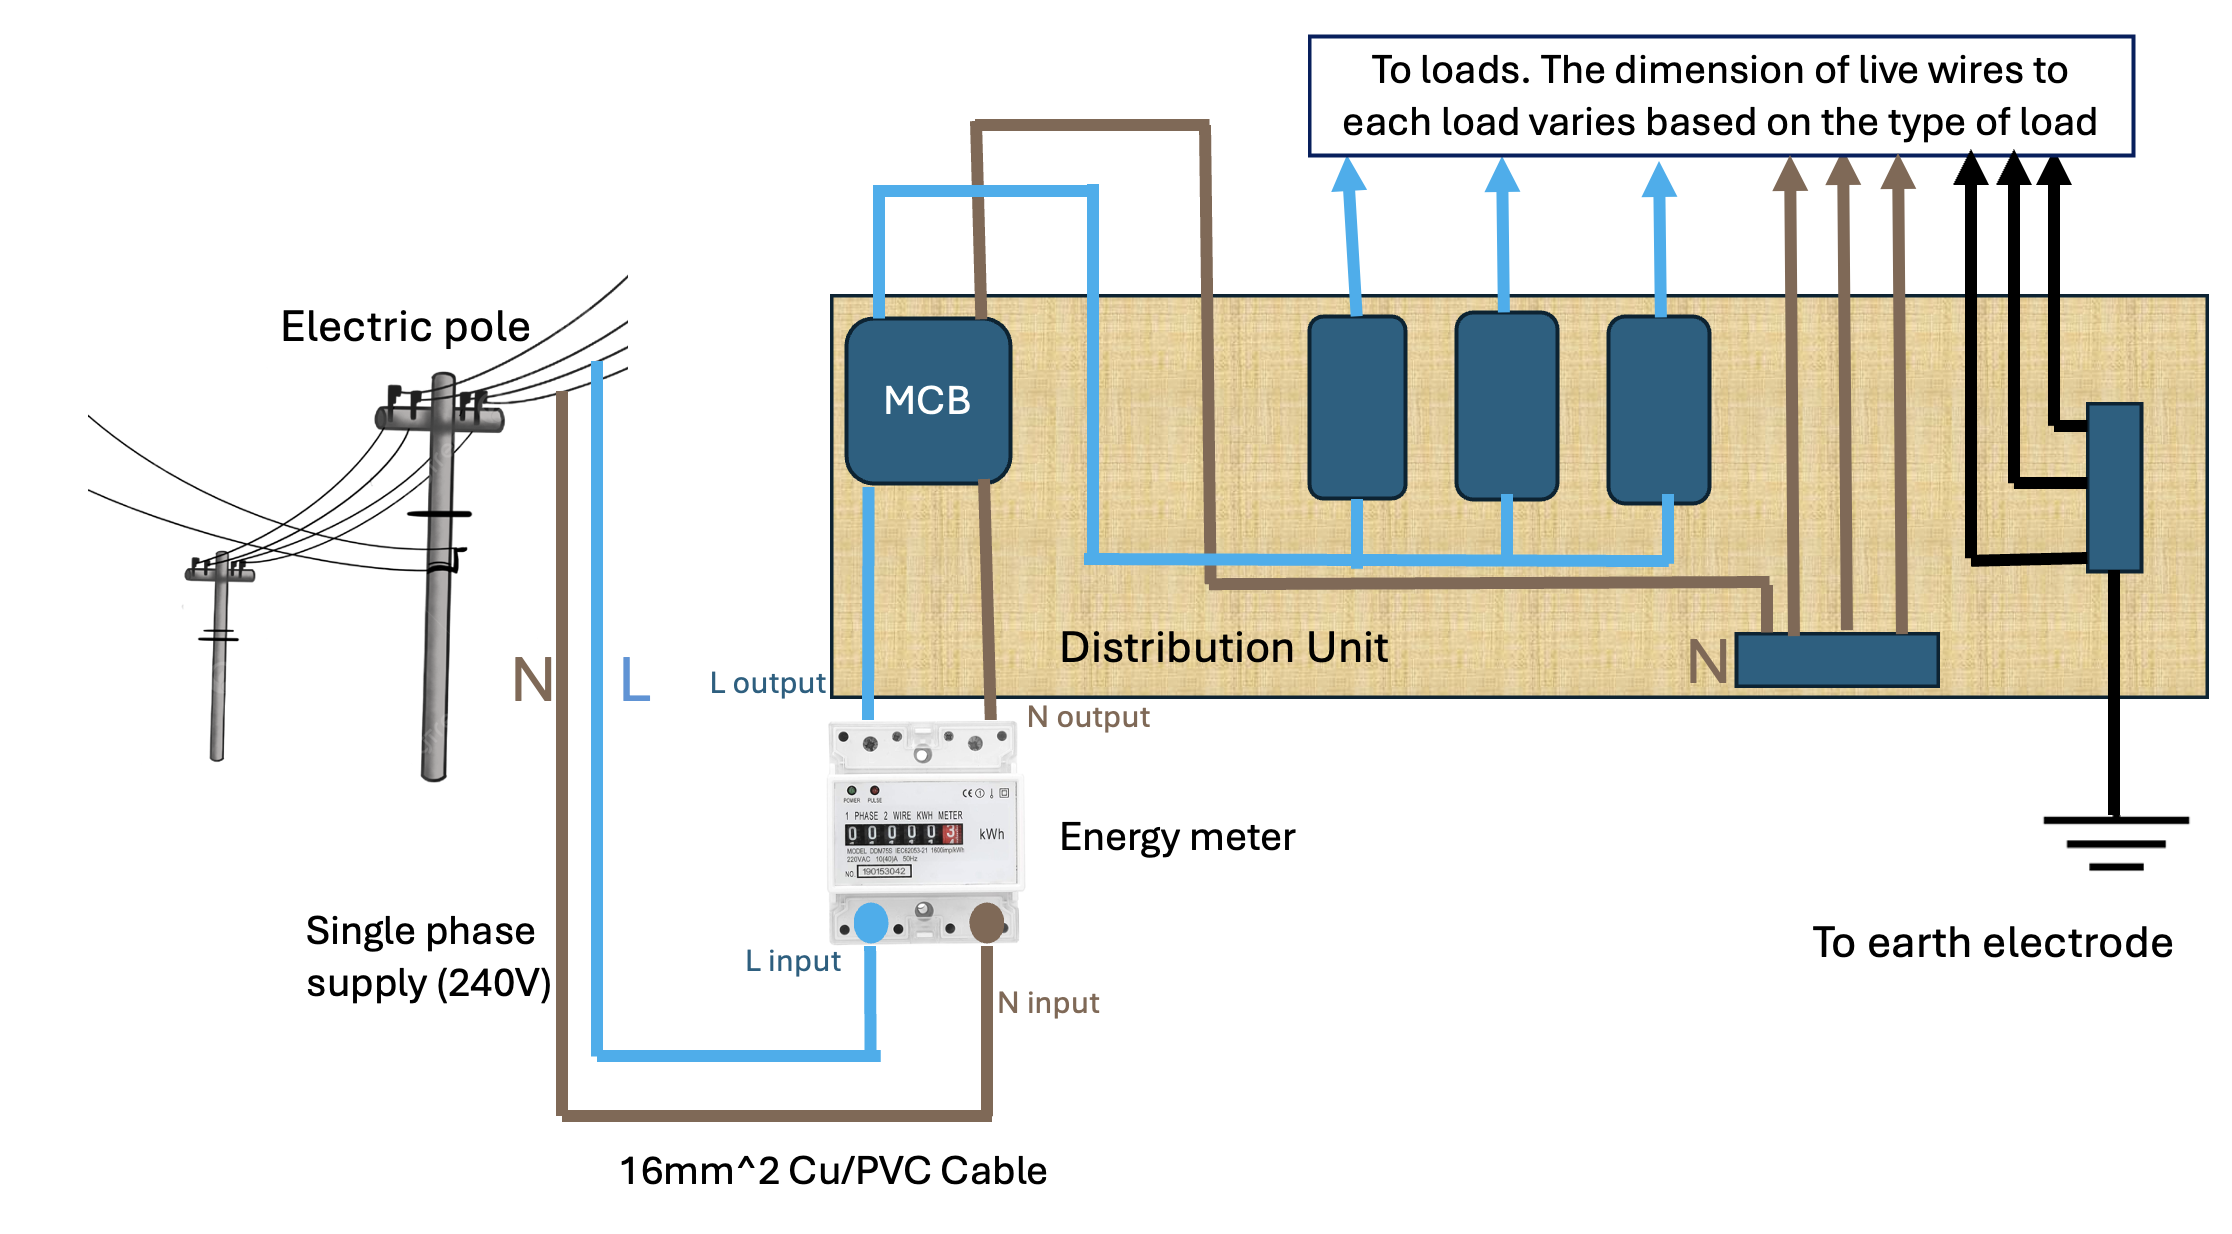
\includegraphics[width=\textwidth]{Wiring/case1_wiring.png}
        \caption{Case 1: A metered connection}
    \end{subfigure}
    \hfill
    \begin{subfigure}[b]{0.32\textwidth}
        \centering
        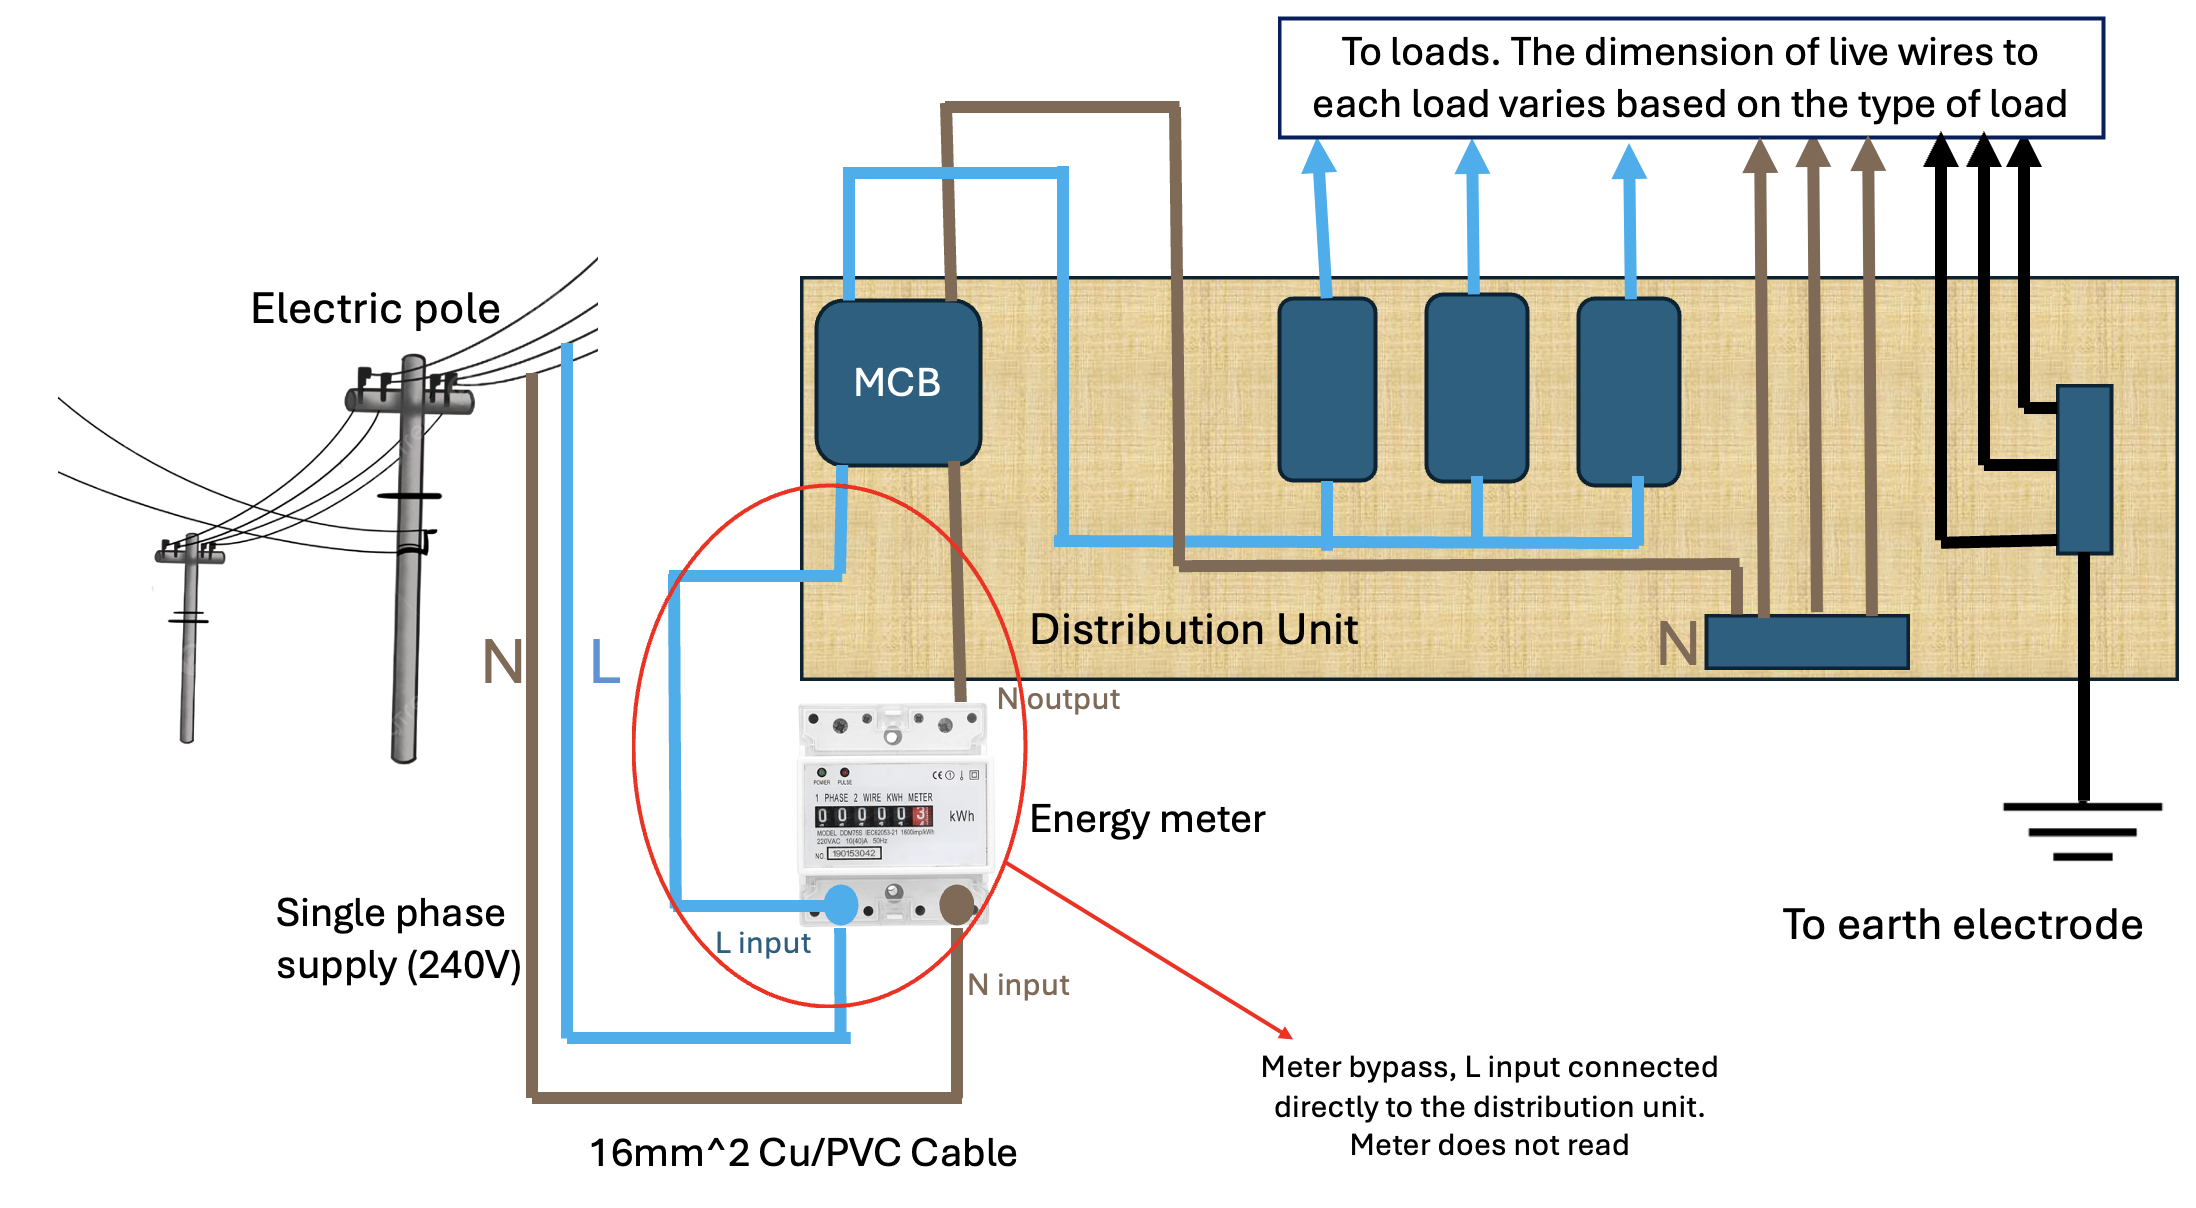
\includegraphics[width=\textwidth]{Wiring/case2_wiring.png}
        \caption{Case 2: Meter bypass, unmetered}
    \end{subfigure}
    \hfill
    \begin{subfigure}[b]{0.32\textwidth}
        \centering
        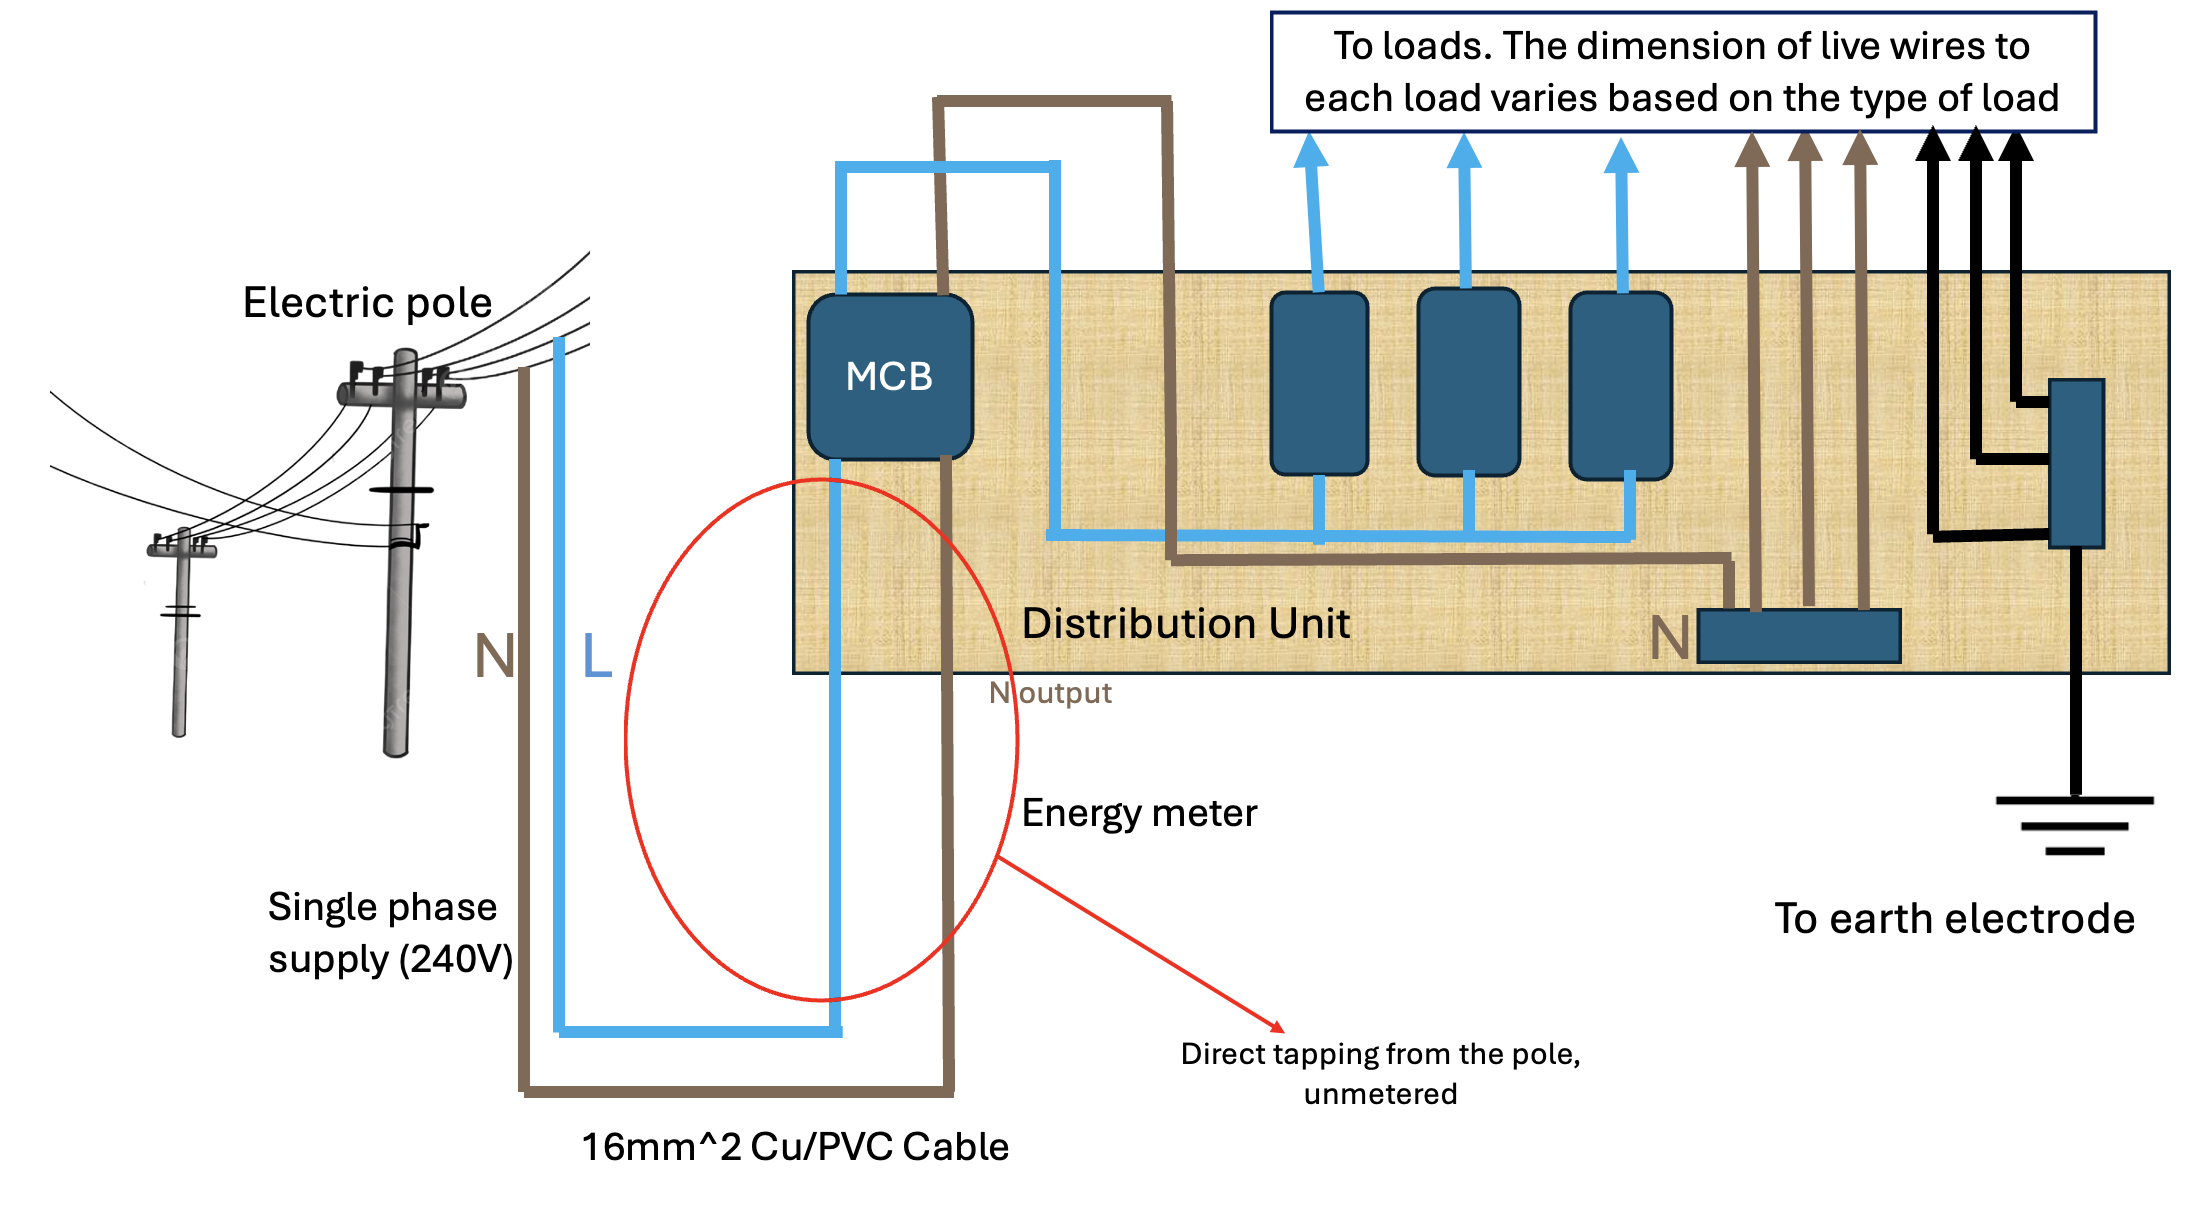
\includegraphics[width=\textwidth]{Wiring/case3_wiring.png}
        \caption{Case 3: Alternate wiring scenario}
    \end{subfigure}

    \caption{Three examples of grid configurations in informal settlements.}
    \label{fig:grid_configs}
\end{figure}

\subsection{Household-Level Consequences of Sustained Voltage Deviations}

While the preceding sections describe the structural and regulatory context of voltage deviations, their significance becomes most apparent at the household level. Empirical evidence from Sub-Saharan Africa documents substantial appliance damage associated with poor voltage quality. In Accra, Ghana, a survey of 2001 grid-connected households and businesses found that 26\% reported appliance damage attributed to poor power quality within the previous month. Enterprises surveyed in Tanzania similarly identified voltage fluctuations and unstable supply conditions as contributors to equipment failure [cite].

These findings align with evidence from our wiring inspections and infrastructure assessment study. Approximately 30\% of participating households reported that appliances had been damaged while plugged in or in use during the preceding month. The most frequently affected devices included electric kettles, refrigerators, protective devices, televisions, sockets, and electric lamps, collectively accounting for more than 70\% of reported failures. Renters reported higher rates of appliance damage than homeowners, suggesting differential exposure to wiring quality, connection configuration, and transformer loading conditions.

Sustained voltage deviations therefore translate structural distribution constraints into tangible equipment stress and economic cost at the point of connection. Understanding not only the occurrence but also the persistence of such voltage states is central to evaluating the functional quality of electricity supply in underserved urban environments.




\clearpage
\FloatBarrier

\begin{figure}[H]
    \centering

    % -------- First Row --------
    \begin{subfigure}[b]{0.3\textwidth}
        \centering
        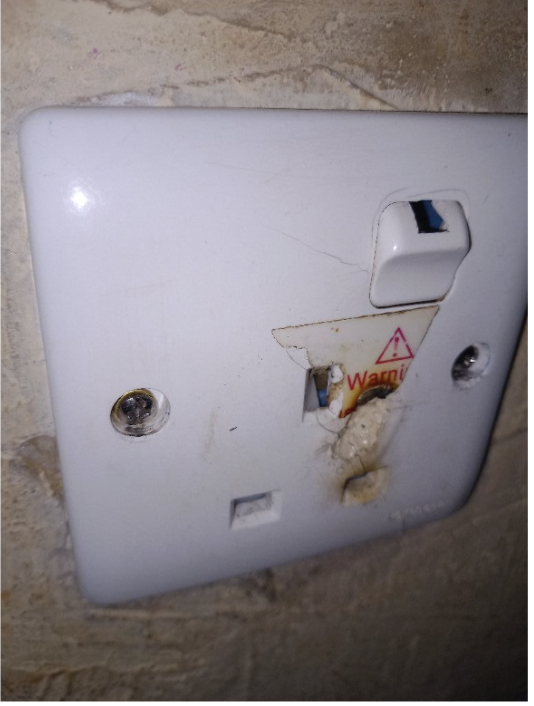
\includegraphics[width=\textwidth]{wiring_images/image1.png}
        \caption{Burnt plug-in use}
    \end{subfigure}
    \hfill
    \begin{subfigure}[b]{0.3\textwidth}
        \centering
        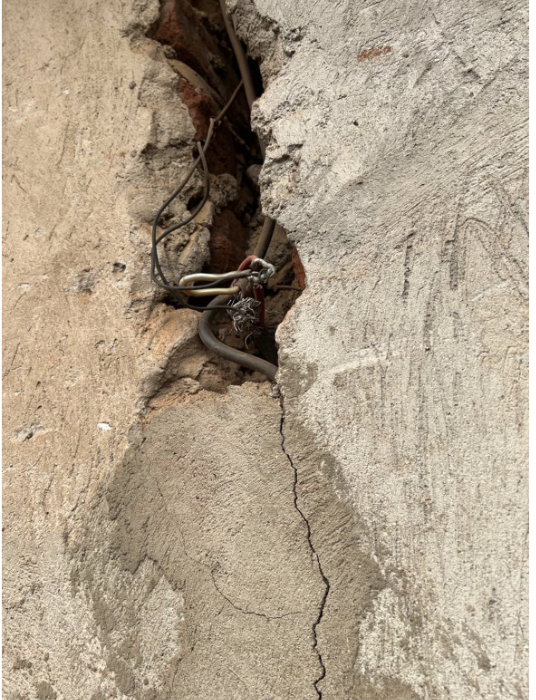
\includegraphics[width=\textwidth]{wiring_images/image2.png}
        \caption{Missing termination box and uninsulated wire connections}
    \end{subfigure}
    \hfill
    \begin{subfigure}[b]{0.3\textwidth}
        \centering
        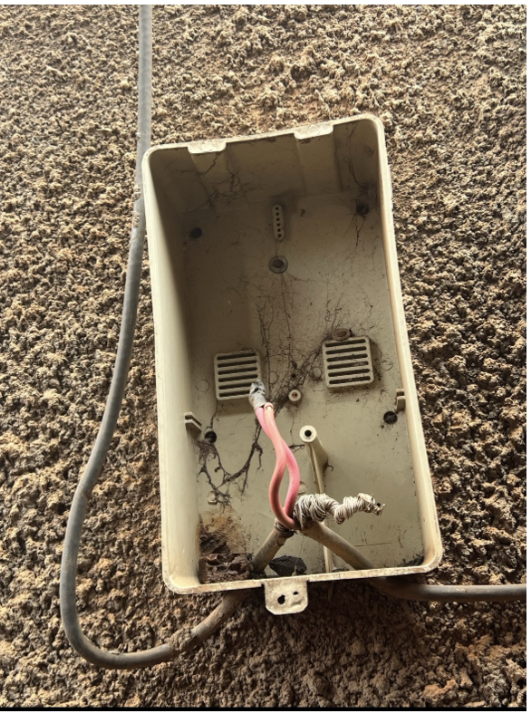
\includegraphics[width=\textwidth]{wiring_images/image3.png}
        \caption{Open meter box and uninsulated wire connections}
    \end{subfigure}

    \vspace{0.5cm}

    % -------- Second Row --------
    \begin{subfigure}[b]{0.3\textwidth}
        \centering
        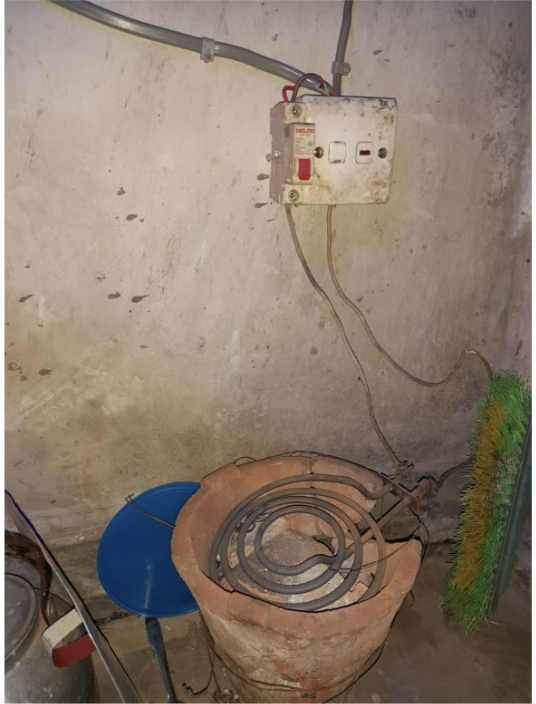
\includegraphics[width=\textwidth]{wiring_images/image4.png}
        \caption{Poorly wired cooking coil}
    \end{subfigure}
    \hfill
    \begin{subfigure}[b]{0.3\textwidth}
        \centering
        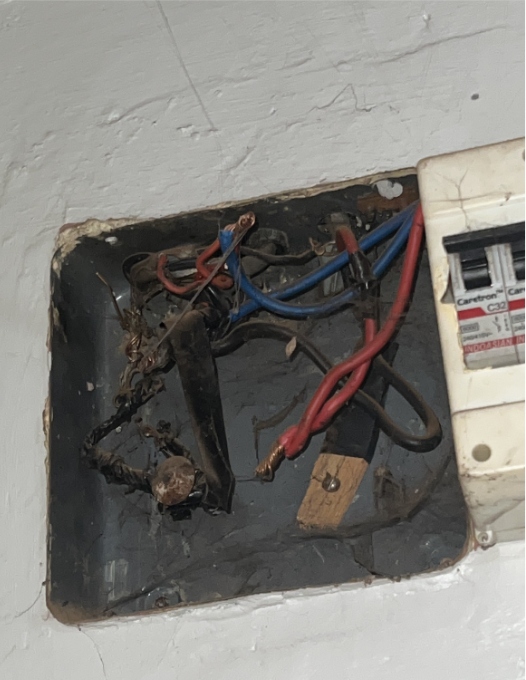
\includegraphics[width=\textwidth]{wiring_images/image5.png}
        \caption{Distribution board missing cover. Live wire uninsulated.}
    \end{subfigure}
    \hfill
    \begin{subfigure}[b]{0.3\textwidth}
        \centering
        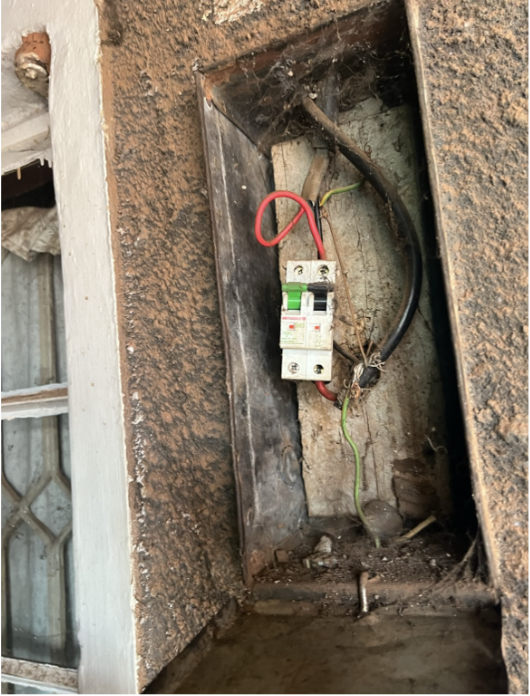
\includegraphics[width=\textwidth]{wiring_images/image6.png}
        \caption{Meter box missing cover}
    \end{subfigure}

    \vspace{0.5cm}

    % -------- Third Row --------
    \begin{subfigure}[b]{0.3\textwidth}
        \centering
        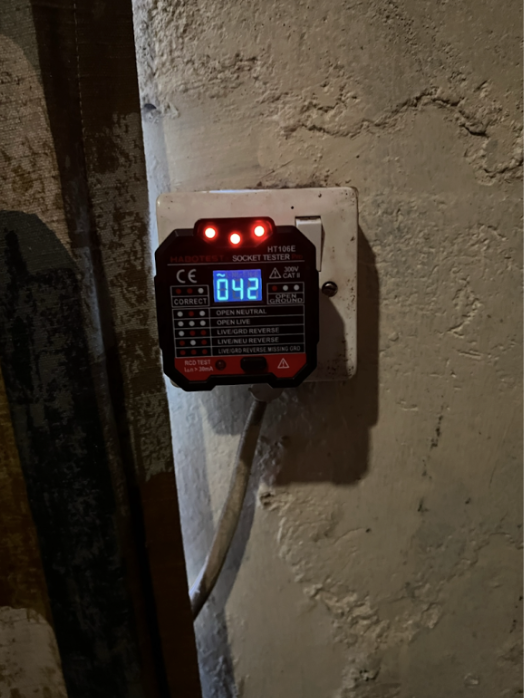
\includegraphics[width=\textwidth]{wiring_images/image7.png}
        \caption{Live/Ground reverse, missing ground}
    \end{subfigure}
    \hfill
    \begin{subfigure}[b]{0.3\textwidth}
        \centering
        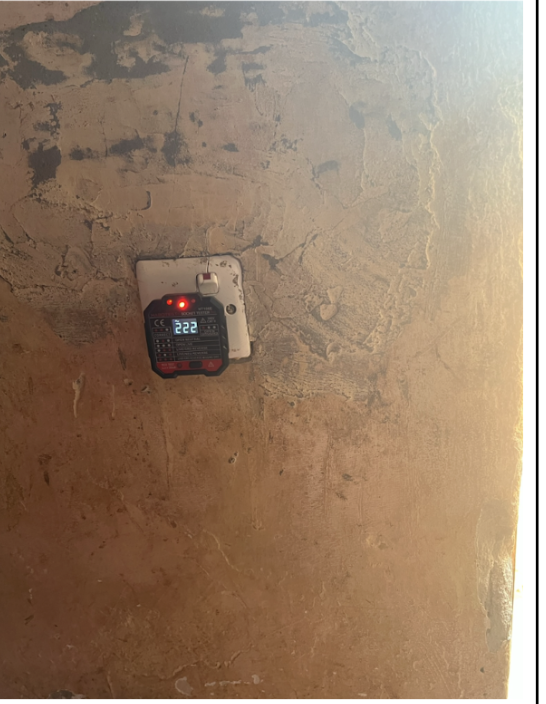
\includegraphics[width=\textwidth]{wiring_images/image8.png}
        \caption{Open neutral}
    \end{subfigure}
    \hfill
    \begin{subfigure}[b]{0.3\textwidth}
        \centering
        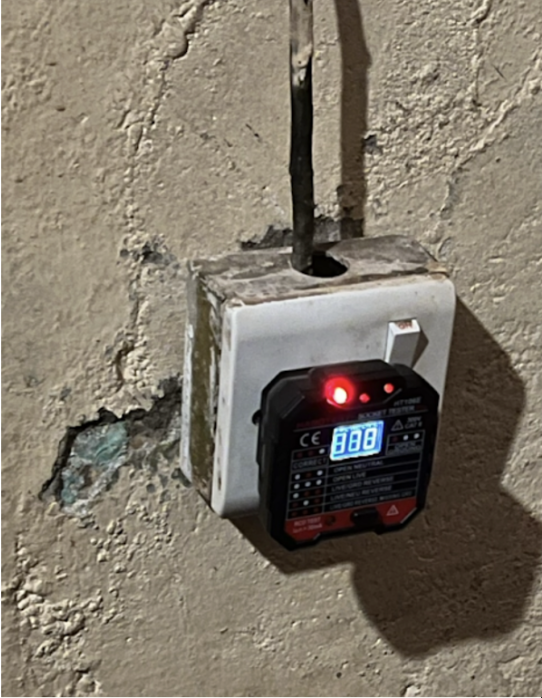
\includegraphics[width=\textwidth]{wiring_images/image9.png}
        \caption{Open ground}
    \end{subfigure}

    \caption{Images showing examples of poor wiring in informal settlements.}
    \label{fig:grid_of_images}
\end{figure}

\FloatBarrier


\section{Methodology}
\label{sec:method}

\subsection{Selection of Measurement Sites}
The voltage quality study is a subset of work done under the broader Spotlight Kampala initiative that seeks to understand energy inequities in urban informal settlements of Kampala using a mixed method approach of interviews, surveys, community forums and remote power quality monitoring [cite]. It is a collaborative initiative involving academic institutions, social scientists, engineers, community leaders, and local organizations focused on slum development \cite{spotlightkampala}.
 

As part of this initiative, data on approximately 60 informal settlements in Kampala were collected in partnership with ACTogether Uganda  and the National Slum Dwellers Federation of Uganda. We integrated these data with satellite imagery to clearly delineate settlement boundaries. From the 60 informal settlements, 25 were randomly selected using probability proportional to size (PPS) sampling. In this approach, settlements were assigned selection probabilities based on their estimated population sizes, such that larger settlements had proportionally higher probabilities of being selected. This ensured that the sample reflected the distribution of population across informal settlements in Kampala. Figure~\ref{fig:kampala_layout} provides the geographic context and spatial layout of the informal settlements.


Proprietary data on transformer and feeder locations within these areas were obtained from the former electricity utility Umeme Limited. Using this dataset, we mapped transformer locations for each of the 25 selected settlements. In collaboration with local field engineers, we identified households and businesses connected to a randomly selected transformer in each informal settlement. This involved physically tracing power lines from the transformers to the connected premises.

For each selected settlement, we recruited six participants: four from the informal settlement and two from a nearby formal settlement. In each settlement type, we identified a specific transformer feeding that settlement and recruited participants whose households were connected to that transformer. The informal and formal transformers were selected such that both were connected to the same distribution feeder, allowing us to control for upstream supply conditions. This design enabled a direct comparison of local voltage quality across settlement types while holding feeder-level grid characteristics constant. The allocation of six participants per site was determined by project funding constraints and the number of available power quality sensors. In total, 150 sensors were deployed: 100 in informal settlements and 50 in formal settlements.

 The goal in each settlement was to recruit four participants connected to a transformer within the informal settlement and two participants connected to a different transformer in a nearby formal settlement. Each participant completed a structured household survey capturing overall grid experience, perceptions of reliability, frequency of outages or voltage fluctuations, and time-of-day patterns of voluntary power disconnection or appliance shutdown. For each informal–formal pair, we selected one transformer in each settlement such that both transformers were connected to the same distribution feeder, allowing for a robust comparison within each community by controlling for upstream supply conditions. The allocation of six participants per site was determined by funding availability and the number of power quality sensor devices available for the study. Across the 25 selected settlements, we recruited 150 participants in total, deploying 100 sensors in informal settlements and 50 in formal settlements. The purpose of recruiting participants in both formal and informal settlements was to compare voltage quality between the two settlement types.  

 Sensor deployment occurred in two phases: the first in 12 communities from October to December 2022, and the second in 13 communities from January to March 2023. The sensors, supplied by nLine, were capable of measuring voltage, frequency, and power availability (including outages caused by utility failures, landlord shut-offs, or depleted pre-paid meters) \cite{nline}
. Each sensor was plugged into a household power outlet for a two-month monitoring period. To mitigate the inconvenience of occupying an outlet and ensure continuous sensor data, participants were provided with an extension board as compensation. Figure~\ref{fig:deployment_setup} shows a schematic of the sensor deployment setup.

 \begin{figure}[H]
    \centering
    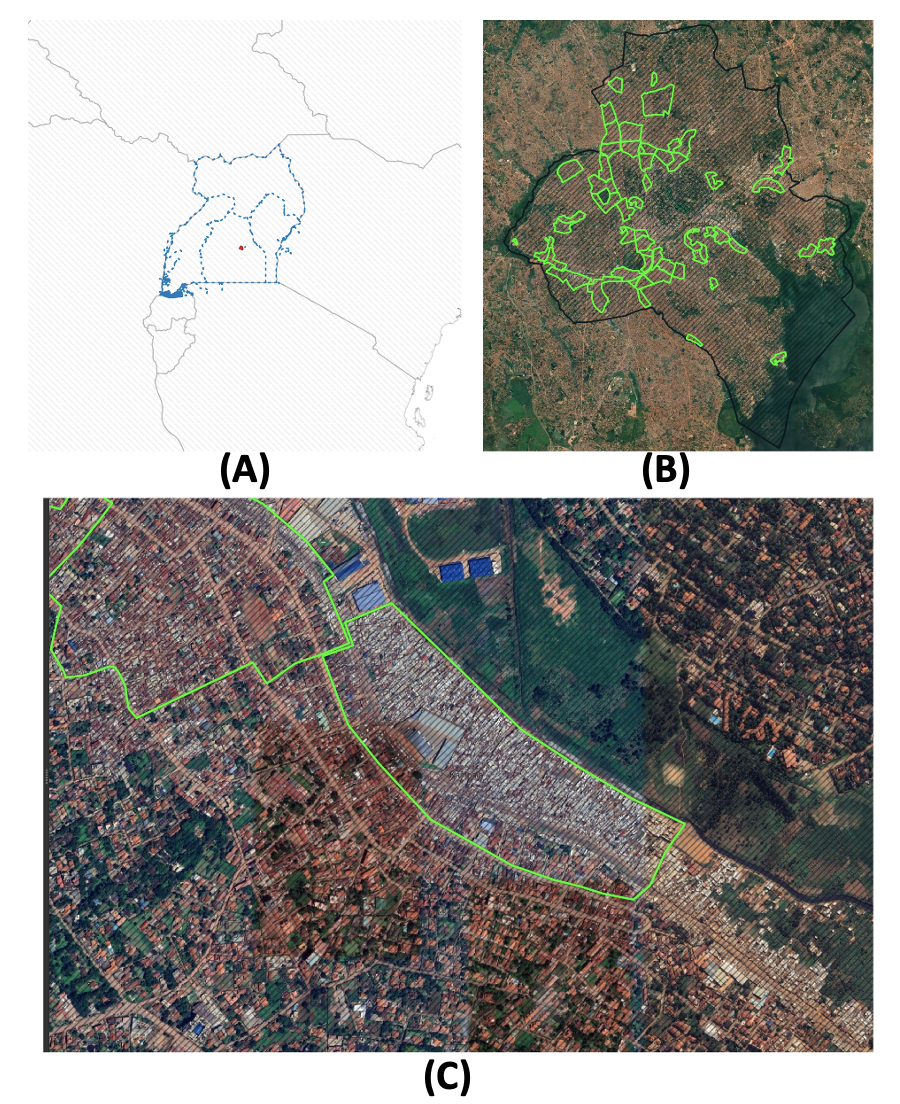
\includegraphics[width=\linewidth]{figures/pq_paper_map_layout.png}
    \caption{Geographic context and spatial layout of informal settlements in Kampala, Uganda. A: Location of Uganda within East Africa. The red dot shows the location of Kampala. B: The green layouts represent the informal settlements of Kampala. C: Zoomed layout showing the boundaries of one informal site. The area outside the green boundary was considered a formal site }
    \label{fig:kampala_layout}
\end{figure}

 
\begin{figure}[H]
    \centering
    
\includegraphics[width=\linewidth]{figures/deployment_schematic.png}
    \caption{Schematic of Sensor Deployment Setup Across Formal and Informal Settlements. Each H is a house or business connected to the selected transformer (T1/T2) in either the formal or informal settlement.}
    \label{fig:deployment_setup}
\end{figure}

\begin{comment}
\subsection{Data Analysis}

\subsection{Descriptive analysis of voltage quality and survey data}
We deployed 150 power quality sensors in the 25 communities of interest (100 sensors in informal settlements and 50 in formal settlements). We obtained proprietary data on transformer locations by community in Kampala from the utility. Using this data, we got the geographical location of all transformers in the 25 communities of interest. For each of the 25 communities, we selected one transformer randomly in the informal settlement and another in the nearby formal settlement. The two transformers selected in each settlement type were on the same feeder to allow for robust results between communities. Through purposive sampling, we then selected four participants (homes/businesses) connected to the transformer of interest in each informal settlement and two participants connected to the transformer in the nearest formal settlement. The purpose of selecting participants in both formal and informal settlements was to compare voltage quality between the two settlement types. We installed power quality sensors in the homes/businesses of the selected participants for at least two months. The power quality sensors were supplied by nline and could measure voltage, frequency, and the presence or absence of power (planned or unplanned outages as well as outages resulting from other factors such as landlord shut-offs of power, finished pre-paid meter units, etc).        
Power quality sensors were deployed in two rounds. The first round of sensors was deployed in 12 sampled communities from October to December 2022, and the second round was deployed in 13 communities from January to March 2023.
\end{comment}

\subsection{Persistence and Predictability in Power Quality}

Power quality is not only defined by how often voltage deviates from acceptable ranges, but also by how long households remain in poor voltage conditions once such deviations occur. In capacity-constrained distribution systems, voltage states often exhibit temporal persistence: once a household enters an Unacceptable or Outage condition, it may remain in that state for extended periods. Importantly, persistence in a low-voltage state does not imply stability. Even while remaining within the Unacceptable range, voltage may fluctuate substantially, producing ongoing instability that households experience as flickering lights, reduced appliance performance, or intermittent functionality. Thus, households may face prolonged exposure to power conditions that are both persistent and internally volatile. This combination of sustained deviation and fluctuation has important implications for household well-being, as unstable or insufficient voltage can damage appliances, reduce their operational efficiency, and degrade the reliability of electricity-dependent services.

At each discrete time step, we define the voltage state as a combination of three elements: time of day, duration in the current state, and instantaneous voltage condition. Time of day is discretized into twelve two-hour intervals spanning the 24-hour cycle. Duration is defined as the cumulative uninterrupted time that a household has remained in its current voltage state and is grouped into three classes: 0–2 hours, 2–4 hours, and more than 4 hours. The instantaneous voltage condition is categorized as Usable, Unacceptable, or Outage. The combination of these three components yields a total of 108 distinct composite states (12 time-of-day intervals × 3 duration classes × 3 voltage categories). As a result, the full transition matrix is 108 × 108, where each entry represents the probability of transitioning from one composite state to another.

At each discrete time step \( t \), we define the entire voltage state space as:
\[
x_t = (i_t, d_t, s_t)
\]
where:
\begin{itemize}
    \item \( i_t \in \mathcal{I} \) represents the time-of-day interval at time \( t \). We discretize the 24-hour day into 12 two-hour bins:
    \[
    \mathcal{I} = \{ [0\textnormal{-}2), [2\textnormal{-}4), \ldots, [22\textnormal{-}24) \}
    \]
    \item \( d_t \in \mathcal{D} \) denotes the duration class that describes the length of time a participant has been continuously in the current voltage state:
    \[
    \mathcal{D} = \{ [0\textnormal{-}2) \textnormal{ hours}, [2\textnormal{-}4) \textnormal{ hours}, 4+ \textnormal{ hours} \}
    \]
    \item \( s_t \in \mathcal{S} \) corresponds to the instantaneous voltage state, defined as:
    \[
    \mathcal{S} = \{ \textnormal{Usable}, \textnormal{Unacceptable}, \textnormal{Outage} \}
    \]
\end{itemize}


By combining these temporal and duration characteristics into our voltage state definition, we preserve the first-order Markov property. Specifically, we assume:
\[
p(x_t \mid x_{t-1}, x_{t-2}, \dots) = p(x_t \mid x_{t-1})
\]
This approach allows us to capture essential contextual dynamics, such as time-of-day variations in voltage and the tendency of certain voltage states to persist over longer durations.
We define the transition probability between composite voltage states as:  

\[
p(x_t \mid x_{t-1}) = p(i_t, d_t, s_t \mid i_{t-1}, d_{t-1}, s_{t-1}),
\]

where each state is defined by time of day, duration in the current state, and instantaneous voltage condition. Transition probabilities are estimated empirically from the observational data by counting the frequency of observed transitions between discrete states and normalizing across all possible successor states:

{\color{sjlmutedred}\textbf{[SJL20260305, Suggested Text to be Replaced]}}
\[
\color{sjlmutedred}
p(x_t \mid x_{t-1}) =
\frac{\textnormal{count}(x_{t-1} \rightarrow x_t)}
{\sum_{x'_t} \textnormal{count}(x_{t-1} \rightarrow x'_t)}.
\]
{\color{sjlmutedblue}\textbf{[SJL20260305, Suggested New Text]}}
\[
\color{sjlmutedblue}
\hat{p}(x_t \mid x_{t-1}) =
\frac{\textnormal{count}(x_{t-1} \rightarrow x_t)}
{\sum_{x'_t} \textnormal{count}(x_{t-1} \rightarrow x'_t)}.
\]
{\color{sjlmutedblue}This is the maximum-likelihood estimator (MLE) for discrete transition probabilities. In what follows, we write $p$ in place of $\hat{p}$ for notational convenience.}

{\color{sjlmutedred}\textbf{[SJL20260305, Suggested Text to be Replaced]}}

{\color{sjlmutedred}High self-transition probabilities indicate persistent voltage conditions, while off-diagonal probabilities capture transitions between Usable, Unacceptable, and Outage states across different time-of-day and duration contexts.

To further characterize the structure and stability of voltage dynamics, we compute entropy-based measures of predictability. While transition probabilities quantify persistence at the state level, entropy provides a summary measure of the overall uncertainty in voltage evolution. Lower entropy values indicate more predictable dynamics, whereas higher values reflect greater volatility and unpredictability.

We first compute the conditional entropy of transitions, defined as}
\[
\color{sjlmutedred}
H(X_t \mid X_{t-1}) =
- \sum_{x_{t-1} \in \mathcal{X}} p(x_{t-1})
\sum_{x_t \in \mathcal{X}} p(x_t \mid x_{t-1})
\log p(x_t \mid x_{t-1}),
\]
{\color{sjlmutedred}which measures the average uncertainty of the next voltage state given the current state. This metric captures the inherent stochasticity of the process after conditioning on time interval, duration class, and voltage condition. Lower values indicate stronger persistence and more structured dynamics, whereas higher values indicate more frequent and less predictable transitions.}

{\color{sjlmutedblue}\textbf{[SJL20260305, Suggested New Text]}}

{\color{sjlmutedblue}Because the composite state encodes time-of-day, duration class, and voltage condition jointly, the structure of the transition matrix reflects both deterministic temporal evolution and stochastic voltage dynamics. Consider a system that remains persistently in Usable voltage: once the duration class saturates at 4+ hours, the only change at each time step is the advance of the time-of-day bin. Within a two-hour bin the system remains in the same composite state (a diagonal entry), and at the bin boundary it transitions to the next time-of-day bin with the same voltage condition and saturated duration class (a structured off-diagonal entry). The same regular pattern holds for a system persistently in Outage. In either case, each row of the transition matrix concentrates its probability mass on one or two successor states, and the remaining entries are near zero.

By contrast, when voltage conditions change frequently---for example, short-duration episodes of Unacceptable voltage interspersed with brief recoveries to Usable---the system cycles through many duration classes and voltage labels at various times of day. This spreads the empirical conditional probability mass across a larger set of off-diagonal entries in each row, reflecting less structured and less predictable dynamics.

The conditional entropy $H(X_t \mid X_{t-1})$ formalizes this distinction. For each source state $x_{t-1}$, we first evaluate the Shannon entropy of that row's conditional distribution $p(\cdot \mid x_{t-1})$, which measures how many successor states carry appreciable probability. These per-row entropies are then averaged over all source states, weighted by the stationary distribution $p(x_{t-1})$:}
\[
\color{sjlmutedblue}
H(X_t \mid X_{t-1}) =
- \sum_{x_{t-1} \in \mathcal{X}} p(x_{t-1})
\sum_{x_t \in \mathcal{X}} p(x_t \mid x_{t-1})
\log p(x_t \mid x_{t-1}).
\]
{\color{sjlmutedblue}When the system is persistent, each row's entropy is low because probability is concentrated on very few successors; the weighted average is therefore low. When the system undergoes frequent, short-duration state changes, each row's entropy is higher because probability is dispersed across many successors; the weighted average rises accordingly. A higher value of $H(X_t \mid X_{t-1})$ therefore indicates that, on average, knowing the current composite state leaves more residual uncertainty about the next state---the voltage process is less predictable.}

We also compute the joint entropy of consecutive states

\[
H(X_t, X_{t-1}) =
- \sum_{x_{t-1} \in \mathcal{X}}
\sum_{x_t \in \mathcal{X}}
p(x_t, x_{t-1}) \log p(x_t, x_{t-1}),
\]

where the joint distribution is given by

\[
p(x_t, x_{t-1}) =
p(x_t \mid x_{t-1}) \, p(x_{t-1}).
\]

This measure accounts for both the uncertainty in the distribution of voltage states and the variability in transitions between them. Together, the transition probabilities and entropy measures provide a comprehensive characterization of persistence, volatility, and predictability in household power quality dynamics.

\begin{comment}

\subsection{Interpretation}

Together, these entropy metrics allow us to rigorously quantify the stochasticity of grid state dynamics in our study region. The conditional entropy \( H(X_t \mid X_{t-1}) \) serves as our primary measure of predictability, indicating how much uncertainty remains about the next state after accounting for the current state. The joint entropy \( H(X_t, X_{t-1}) \) provides an additional layer of insight by encapsulating the overall system complexity, including both state diversity and transition uncertainty.

We use these measures to compare different regions, seasons, or intervention scenarios, providing actionable insights into the stability and reliability of energy access.


\subsubsection{Explicit Definition of Conditional Entropy}

For our application, the conditional entropy of the Markov chain over the expanded state space \( x = (i, d, s) \) is given explicitly by:
\[
\begin{aligned}
H(X_t \mid X_{t-1}) 
= \; & - \sum_{i_{t-1} \in \mathcal{I}} \sum_{d_{t-1} \in \mathcal{D}} \sum_{s_{t-1} \in \mathcal{S}} p(i_{t-1}, d_{t-1}, s_{t-1}) \\
& \times \sum_{i_t \in \mathcal{I}} \sum_{d_t \in \mathcal{D}} \sum_{s_t \in \mathcal{S}} p(i_t, d_t, s_t \mid i_{t-1}, d_{t-1}, s_{t-1}) \\
& \times \log p(i_t, d_t, s_t \mid i_{t-1}, d_{t-1}, s_{t-1})
\end{aligned}
\]

This quantity measures the expected uncertainty of the next state \( (i_t, d_t, s_t) \), given knowledge of the current state \( (i_{t-1}, d_{t-1}, s_{t-1}) \).

\subsubsection{Explicit Definition of Joint Entropy}

The joint entropy of two consecutive states in our Markov chain is expressed as:
\[
\begin{aligned}
H(X_t, X_{t-1})
= \; & - \sum_{i_{t-1} \in \mathcal{I}} \sum_{d_{t-1} \in \mathcal{D}} \sum_{s_{t-1} \in \mathcal{S}} \sum_{i_t \in \mathcal{I}} \sum_{d_t \in \mathcal{D}} \sum_{s_t \in \mathcal{S}} \\
& \times p(i_t, d_t, s_t, i_{t-1}, d_{t-1}, s_{t-1}) \\
& \times \log p(i_t, d_t, s_t, i_{t-1}, d_{t-1}, s_{t-1})
\end{aligned}
\]

Given the Markov property, the joint probability factorizes as:
\[
p(i_t, d_t, s_t, i_{t-1}, d_{t-1}, s_{t-1}) = p(i_t, d_t, s_t \mid i_{t-1}, d_{t-1}, s_{t-1}) \cdot p(i_{t-1}, d_{t-1}, s_{t-1})
\]
The joint entropy quantifies the total uncertainty associated with the sequence of two successive states in the system.

\end{comment}
\section{Results}
This section examines voltage variation across the study area, beginning with patterns observed within individual settlements, followed by differences between settlements. It then compares voltage characteristics between formal and informal settlement types, explores variation by connection type and time of day, and assesses voltage \suggestreplacesjl{predictability and entropy-based analysis of voltage quality.}{predictability using a Markov chain voltage quality model and entropy-based predictability measures.}

\label{sec:results}
\subsection{Overview of Voltage Quality Across Settlement Types}
Across the study sites, voltage quality was highly variable, both within and between settlements, with informal areas consistently experiencing poorer power conditions compared to formal neighborhoods. Measured voltages frequently fell outside the acceptable range of 240V ± 6\%, particularly in informal sites.

Within informal settlements, many sites experienced average voltages well below acceptable voltage thresholds throughout the day. Heat maps of the mean hourly voltage (see Figure~\ref{fig:heatmap_joypy}a) show that in many informal settlements, the voltage decreased significantly during peak demand hours between 06:00 and 22:00. These drops were often sustained for several hours at certain times of day (mostly peak hours) and in some cases brought voltages below 210V, which is well outside of standard service thresholds. 

We also observed notable disparities in the quality of voltage supply between settlements. Although some informal sites (e.g., Sites B, C, L, O, U and W) maintained relatively stable voltage levels, others (e.g., Site M, P and V) consistently recorded lower means and wider fluctuations. A ridgeline plot and KDE comparison (see Figure~\ref{fig:heatmap_joypy}b)) showed that some sites had voltage distributions heavily skewed toward under-voltage, while others had bimodal or relatively flat distributions, indicative of instability and inconsistent supply. These differences are not easily explained by geography alone and may reflect underlying grid design or maintenance inequalities across neighborhoods.


Figure~\ref{fig:voltage_distribution_sett_type}a shows the distribution of voltage measurements aggregated by settlement type. The Y axis shows the proportion of voltage samples under each voltage grade. We see more voltage samples within the poor voltage grades (Grades C-F) in the informal settlements than in the formal settlements. The proportion of extremely low voltage (Grade F) is significantly higher in the informal (20\%) than in the formal settlements (~10\%). These extremely low-voltage samples signify power supplies that can barely be used for any end-use. Furthermore, a fitted normal distribution comparing the distribution of voltages across the two settlement types shows that most voltage points in the formal settlements are concentrated within the stated voltage limits with very little spread around the mean (std) as seen in Figure~\ref{fig:voltage_distribution_sett_type}b. Conversely, the voltage distribution in the informal settlements is more spread out and left-skewed, indicating significant voltage variations and deviation from the nominal voltage. Both types of settlements have few measurements beyond the upper voltage limit. %The plane (Vmean, std) further shows how close to the low voltage limit the 10-minute weekly average is with a very high standard deviation. The average 10-minute weekly voltage being closer to the lower voltage bound with a high standard deviation implies there is a higher probability of voltage points straying outside the lower voltage limit. 
\begin{comment}
%\begin{figure}[H]
    \centering
    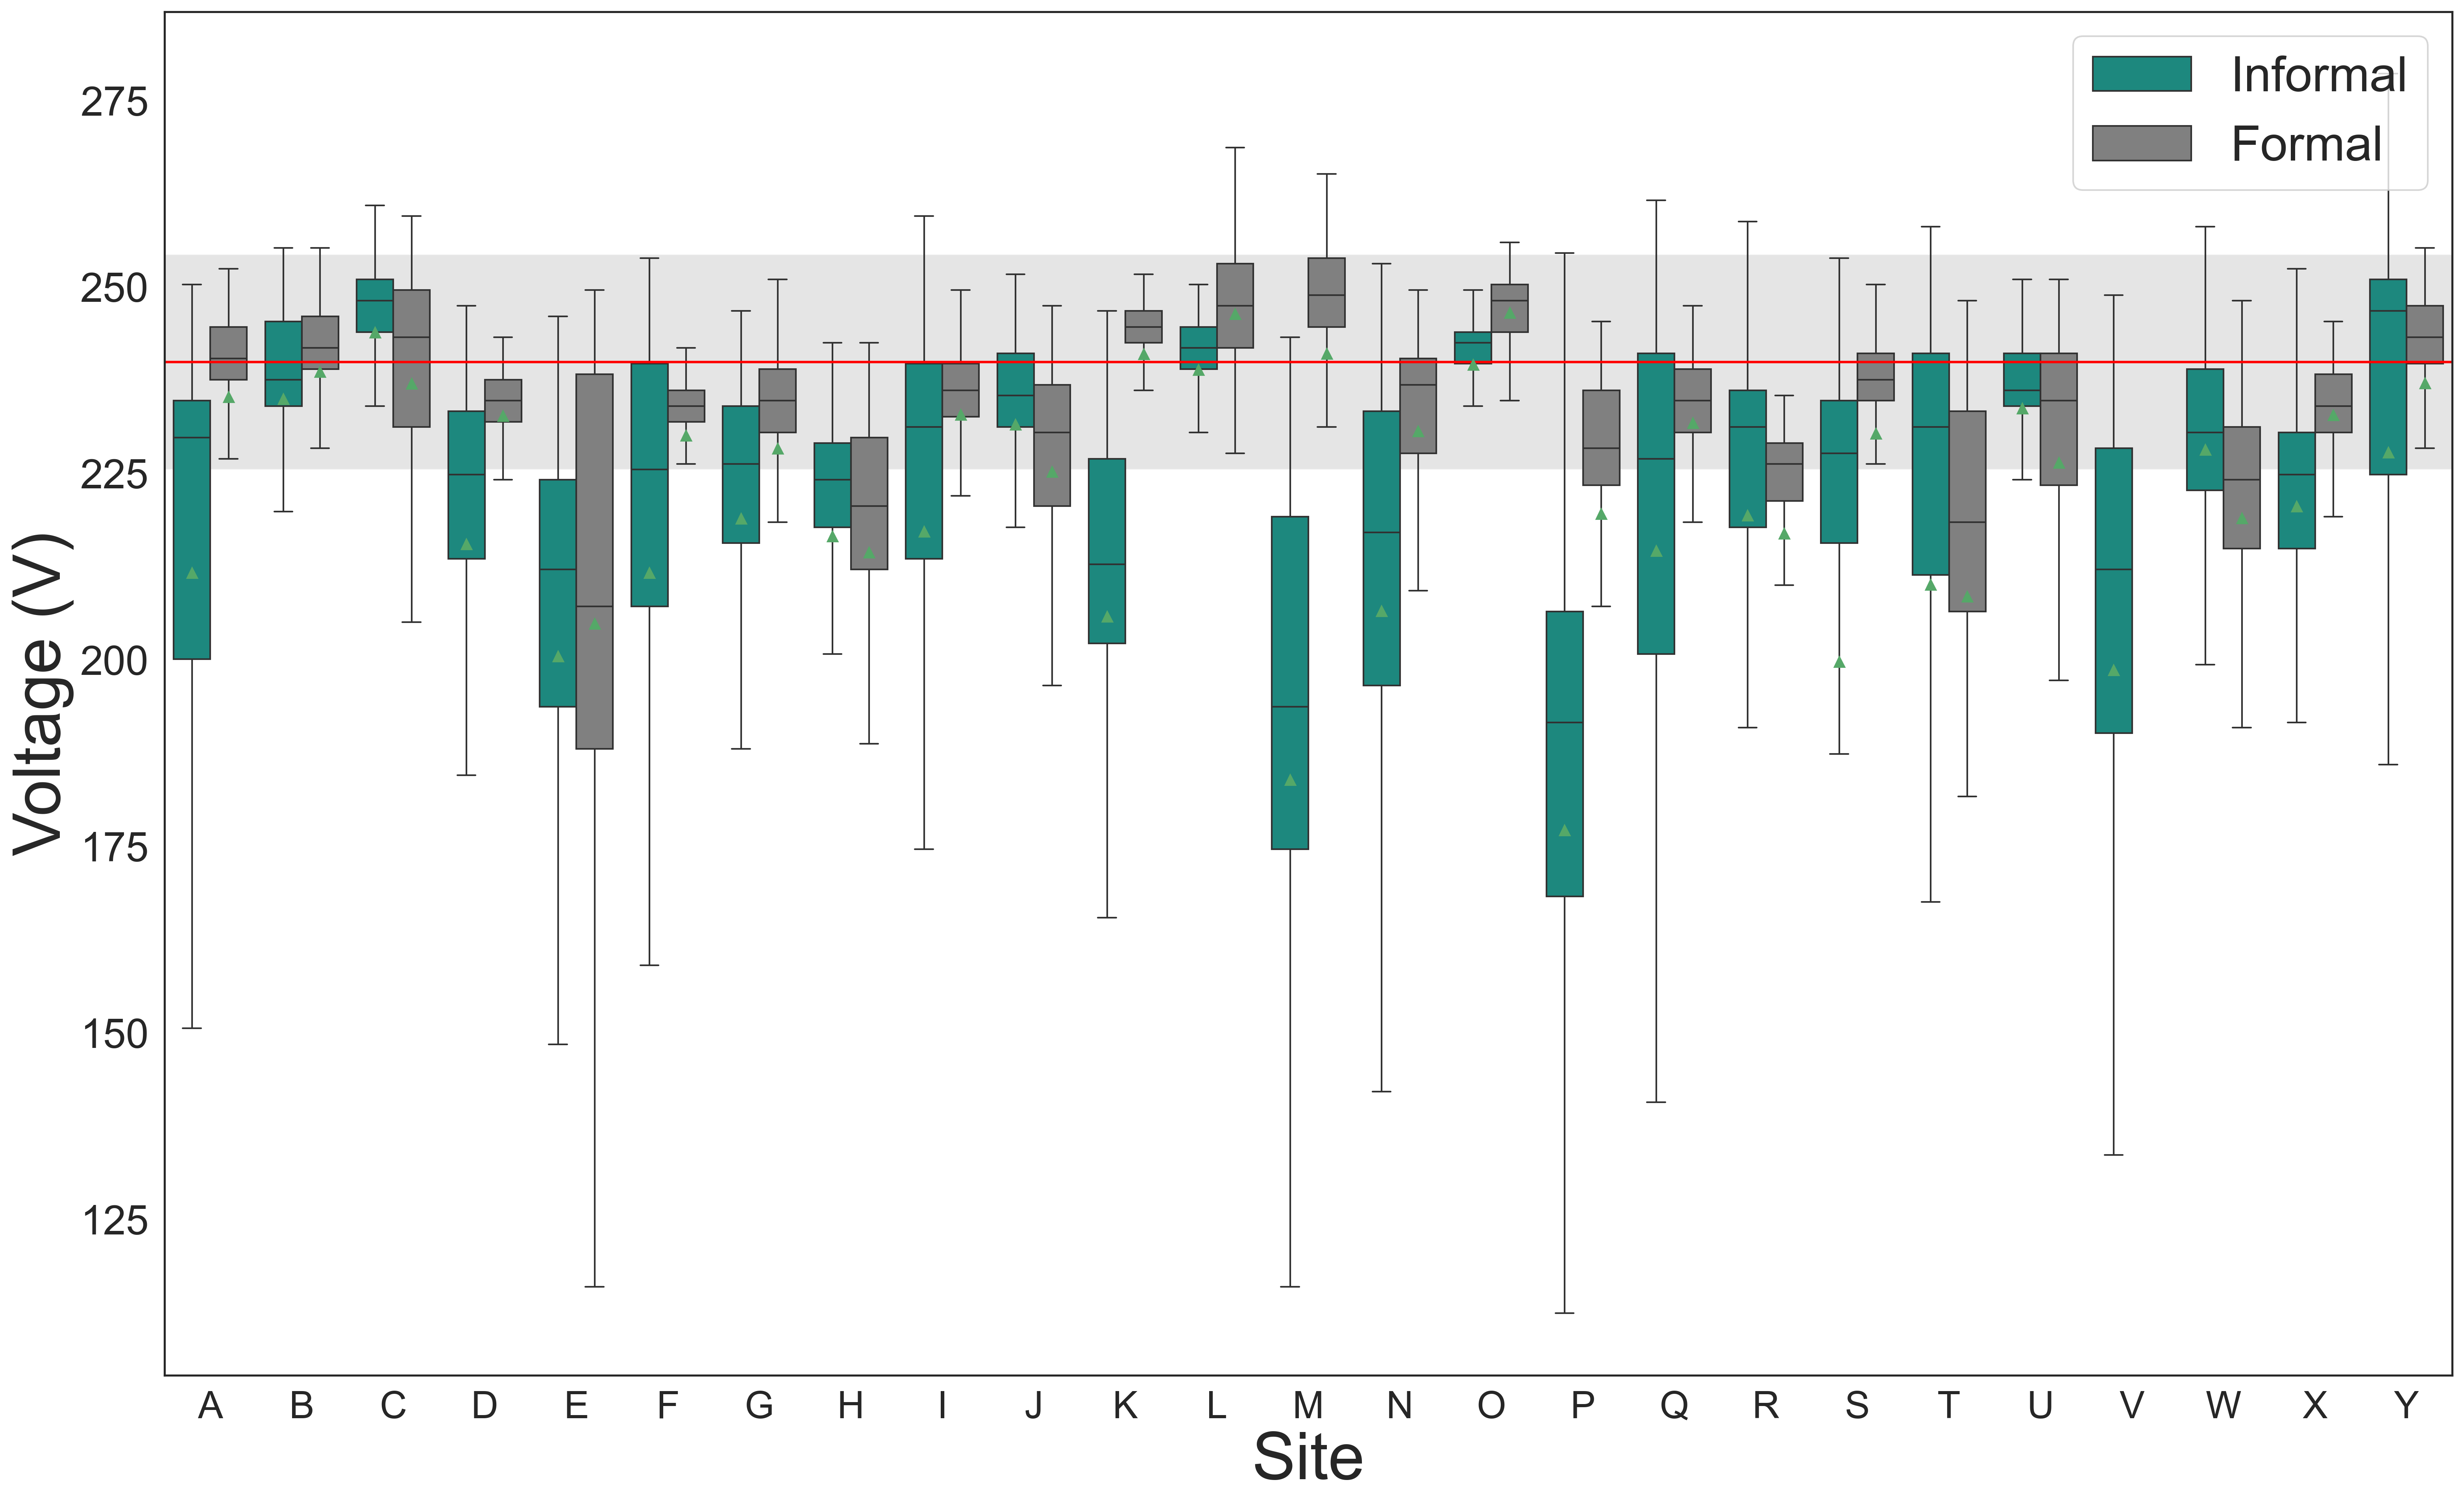
\includegraphics[width=0.9\linewidth]{figures/voltage_by_site.png} % Adjust the width as needed
    \caption{This boxplot compares voltage measurements across 25 anonymized pairs of sites in Kampala (labeled A–Y), disaggregated by settlement type (formal in gray, informal in teal). Each box shows the interquartile range (IQR), with the median marked inside. Whiskers indicate variability outside the upper and lower quartiles, and potential outliers are plotted as individual points. The red horizontal line at 240V represents the nominal RMS voltage standard. The shaded area between 225.6V and 254.4V indicates the ±6\% tolerance band around the nominal voltage as recommended by power quality standards.}
    \label{fig:voltage_distribution_sett_type}
%\end{figure}

\end{comment}

\begin{figure}[H]
    \centering
    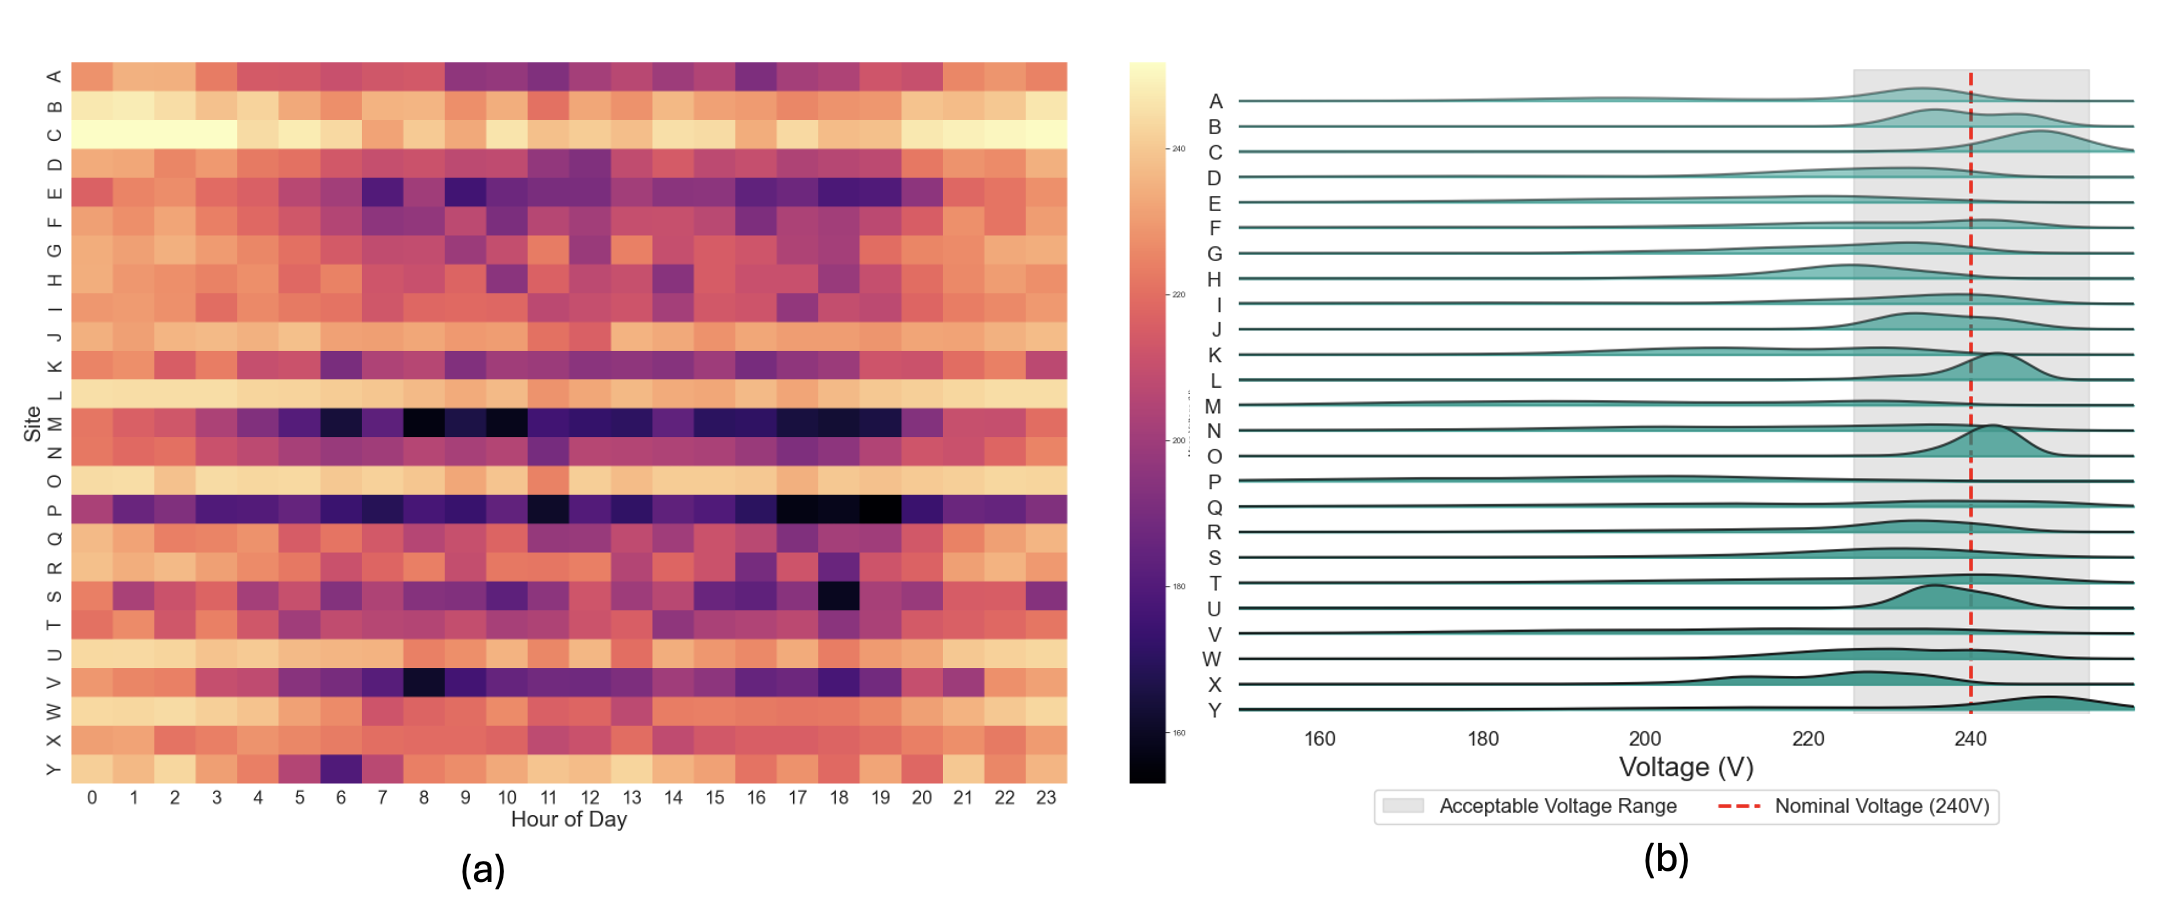
\includegraphics[width=0.9\linewidth]{figures/heatmap_joypy.png} % Adjust the width as needed
    \caption{\textbf{(a)}: Hourly voltage variation across informal settlements. This heatmap shows the mean voltage recorded at each hour of the day across multiple informal settlement sites (labeled A to Y). Each row represents a different settlement, and each column corresponds to an hour (0–23). Warmer colors (yellow–orange) indicate higher average voltages, while darker shades (purple–black) represent lower voltages, \textbf{(b)}: Voltage distribution by site across informal settlements. Each ridge plot represents the kernel density estimation of voltage measurements at a specific informal settlement (labeled A–Y). The dashed red line indicates Uganda's grid's nominal voltage (240V) with the shaded vertical band marking the acceptable voltage range of ± 6\% from nominal.}
    \label{fig:heatmap_joypy}
\end{figure}

\begin{comment}
\begin{figure}[H]
    \centering
    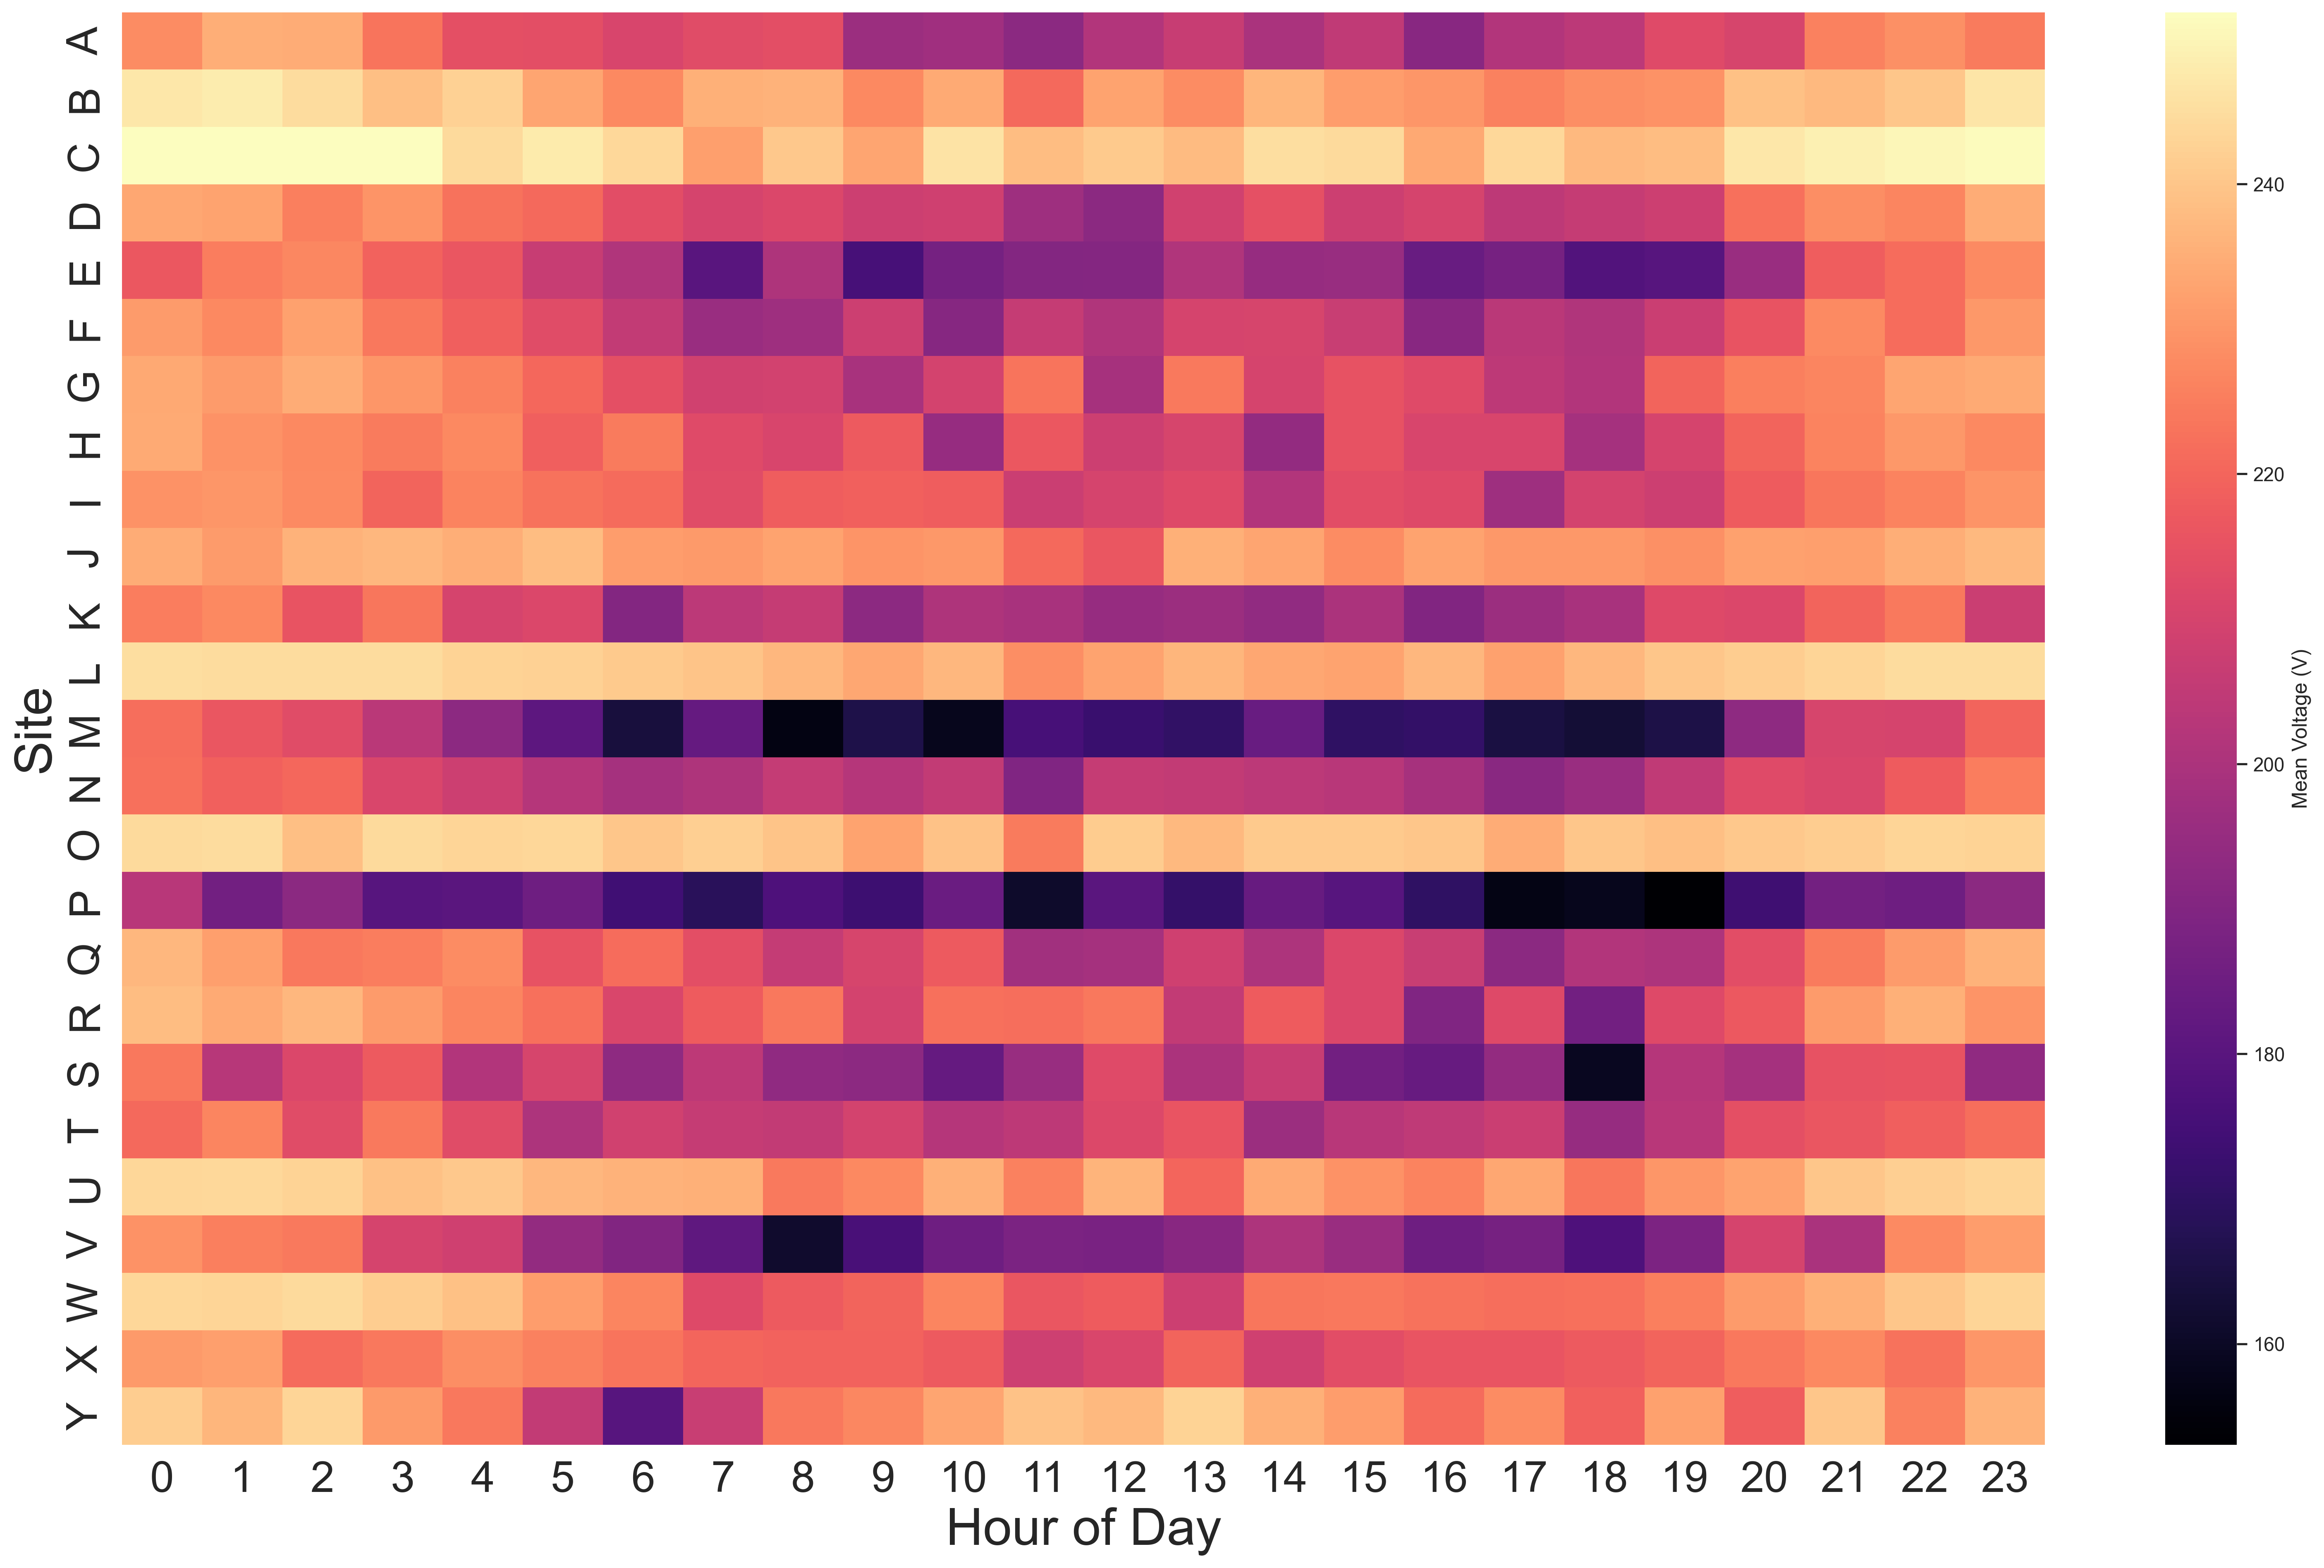
\includegraphics[width=0.9\linewidth]{figures/heat_map_hr_png.png} % Adjust the width as needed
    \caption{Hourly voltage variation across informal settlements. This heatmap shows the mean voltage recorded at each hour of the day across multiple informal settlement sites (labeled A to Y). Each row represents a different settlement, and each column corresponds to an hour (0–23). Warmer colors (yellow–orange) indicate higher average voltages, while darker shades (purple–black) represent lower voltages.}
    \label{fig:heatmap}
\end{figure}

\end{comment}
\begin{figure}[H]
    \centering
    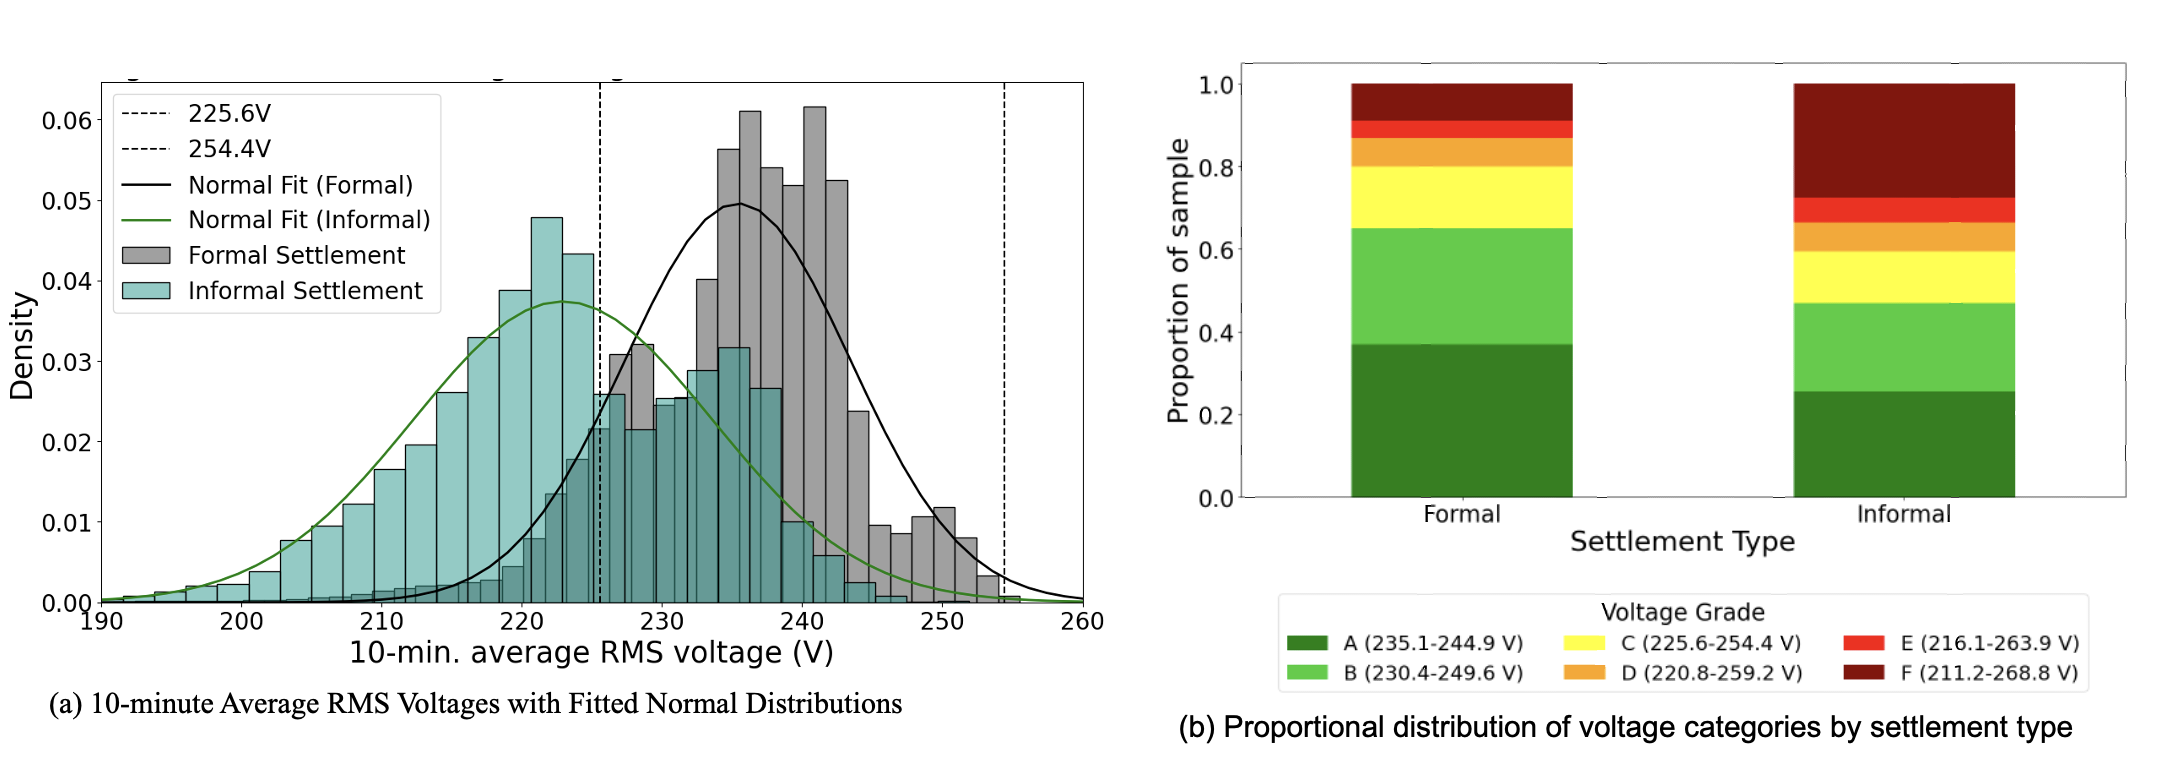
\includegraphics[width=0.9\linewidth]{figures/prob_dis_and_prop_v.png}
    \caption{\textbf{(a)}: 10-minute average RMS voltage distributions by settlement type, with fitted normal curves. This histogram compares the distribution of 10-minute average RMS voltage measurements for formal (gray) and informal (teal) settlements. Overlaid normal distribution curves highlight the differing central tendencies and variances: formal settlements show a higher and more tightly clustered voltage distribution, while informal settlements show a wider and lower distribution, indicating greater variability and potential under-voltage issues. \textbf{(b)}: Proportional distribution of voltage quality grades by settlement type. Each bar represents the share of voltage samples in each voltage quality category (Grades A–F, defined by increasing voltage range thresholds).}
\label{fig:voltage_distribution_sett_type}
\end{figure}

\begin{comment}
    \begin{figure}[H] % Use [H] to enforce exact placement
    \centering
    % First subplot
    \begin{subfigure}[b]{0.48\columnwidth}
        \centering
        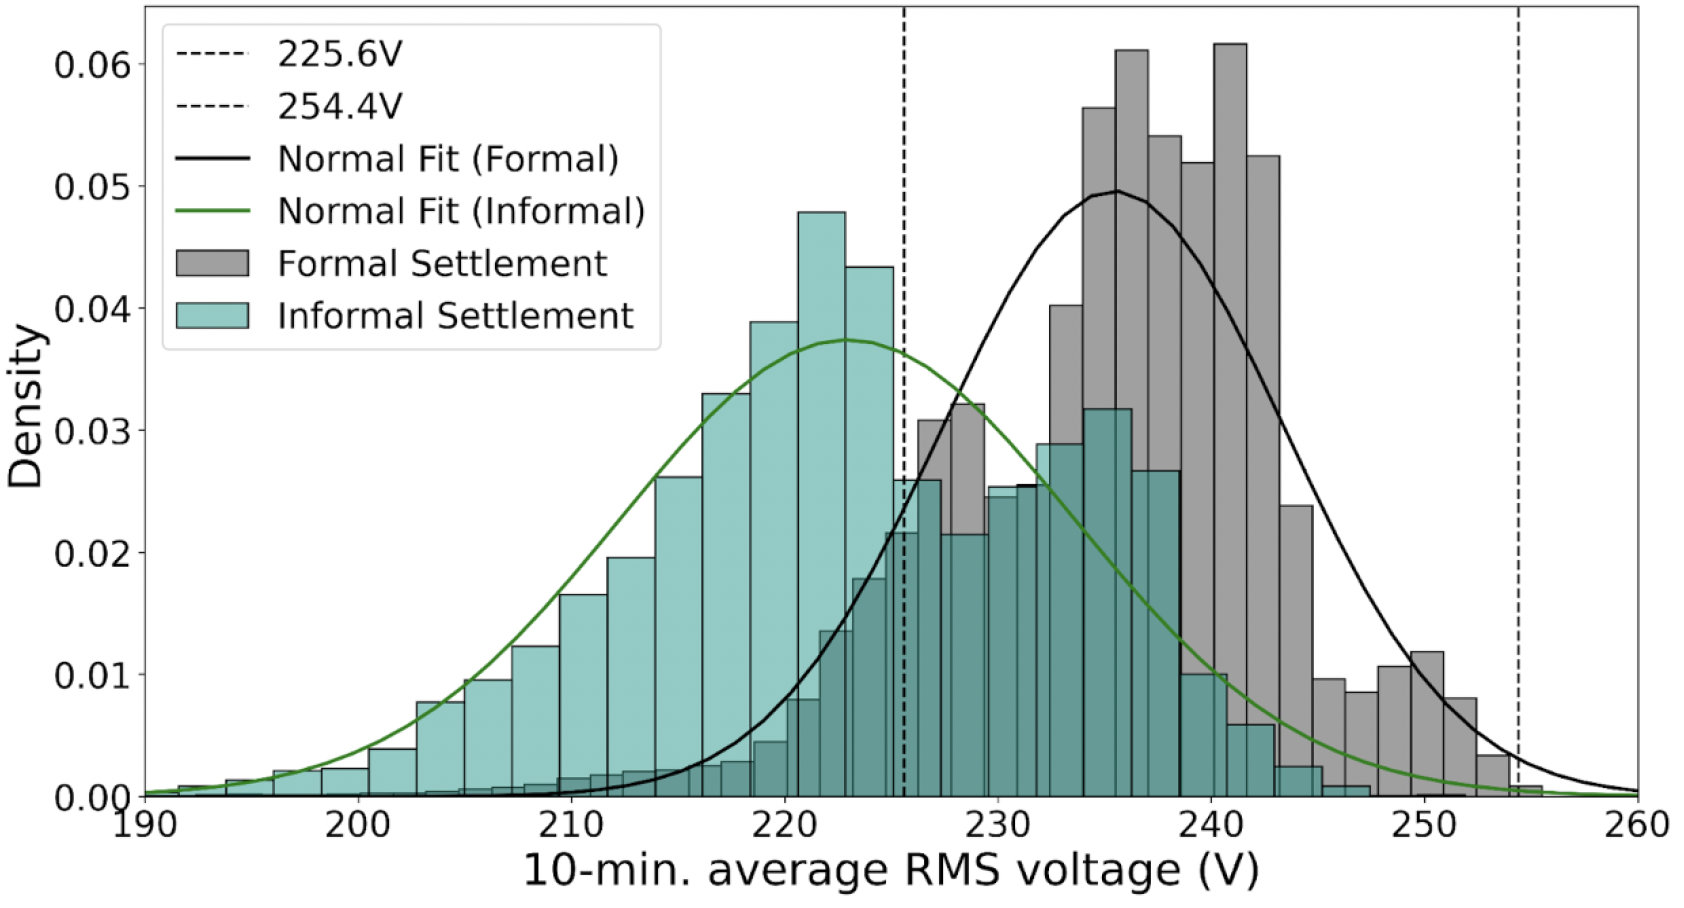
\includegraphics[width=\textwidth]{figures/pdf_voltage.png}
        \caption{10-minute Average RMS Voltages with Fitted Normal Distributions}
        \label{fig:pdf_voltage}
    \end{subfigure}
    \hfill
    % Second subplot
    \begin{subfigure}[b]{0.48\columnwidth}
        \centering
        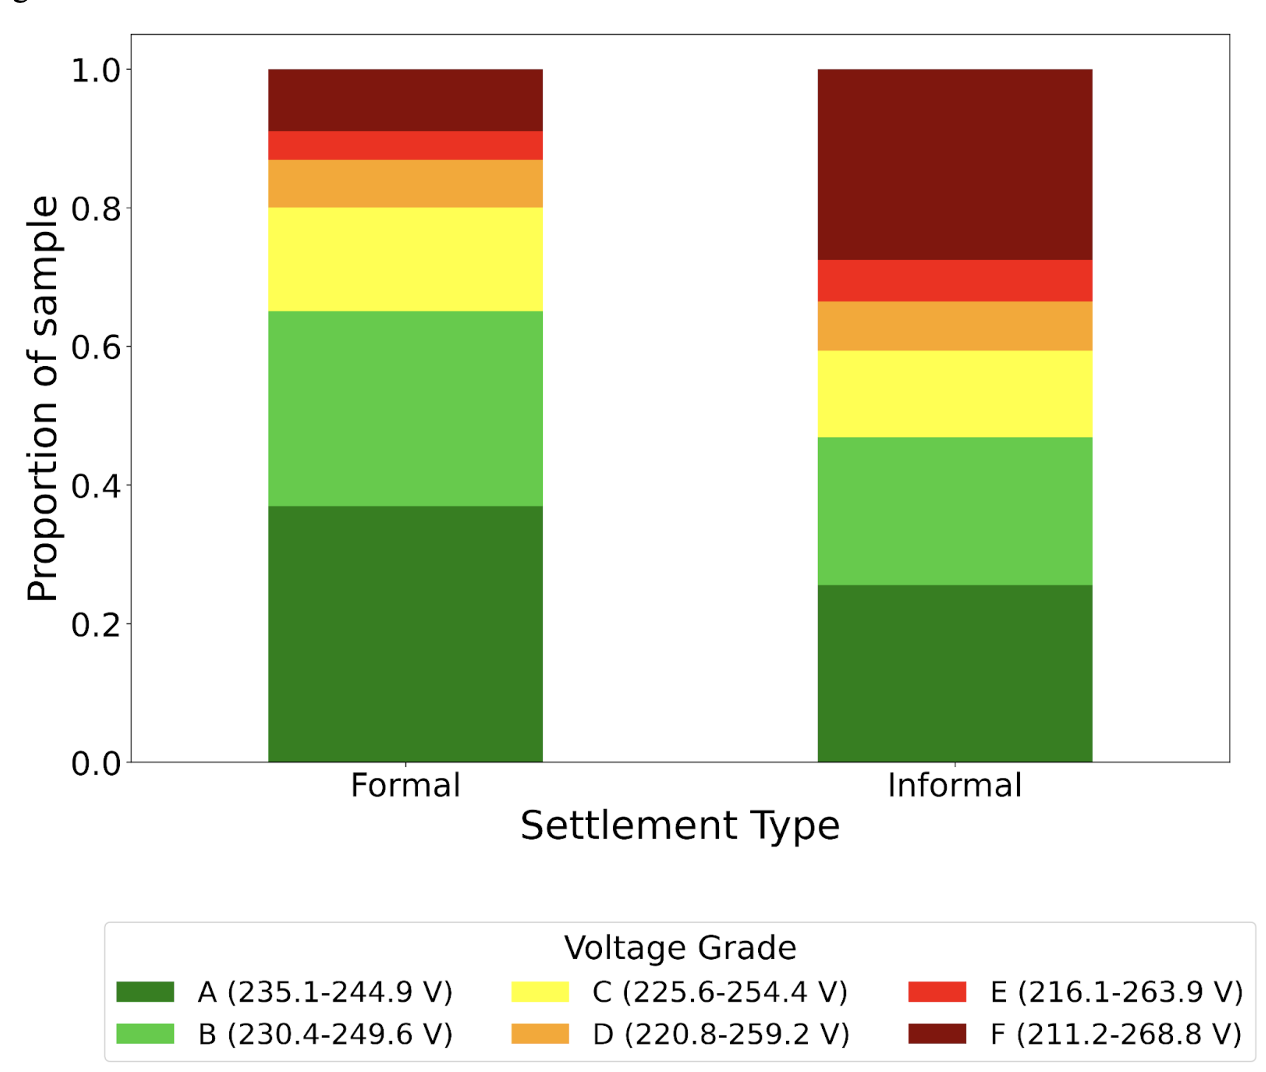
\includegraphics[width=\textwidth]{figures/v_class.png}
        \caption{Proportional distribution of voltage categories by settlement type.}
        \label{fig:v_class}
    \end{subfigure}
    \caption{Voltage distribution across 25 informal settlements, 156 households and small businesses}
    \label{fig:voltage_analysis}
\end{figure}
\end{comment}



\subsection{Voltage quality by connection types} 

Voltage quality varies significantly depending on how a user is connected to the grid, whether through collective metered, individual metered, collective unmetered, or individual unmetered connections. Figure~\ref{fig:pq_bnd} presents the empirical cumulative distribution functions (ECDF) of RMS voltage across these four connection modalities. Users in formal settlements (primarily individuał metered) exhibit the best performance, with 90\% of voltage samples falling within the acceptable range of {240V~$\pm$6\%} (i.e., 225.6–254.4V). In contrast, collective unmetered users in informal settlements experience the poorest quality, with over 70\% of samples falling below 225.6V.

Although metered users in informal settlements (both individual and collective) show improved performance over unmetered users in the same areas, their voltage quality remains significantly worse than the metered users in the formal settlements (baseline). This disparity persists despite both groups being connected to the same feeder, highlighting the role of local infrastructure conditions. The local infrastructure in  informal settlements is often congested and users rely on substandard wiring and fragmented connection setups. These localized weaknesses -- congested infrastructure, degraded conductors, and a lack of uniform installation practices -- undermine voltage quality, even for metered users.

In addition to the connection types, we also investigated the impact of daisy chain position (a proxy for how far a user is from the main connection point in a daisy-chained setup for shared connections) on voltage quality. The rationale is that as electricity travels through successive connections (e.g., from position 1 to 3), voltage may degrade due to increased resistance, poor-quality conductors, or cumulative load. As shown in Figure~\ref{fig:cons_chain}(b), users at chain position 1 typically receive higher and more stable voltage levels compared to those further along the chain. This downward trend in voltage with increasing chain position highlights the compounding effect of informal infrastructure layouts on power quality, especially in densely populated informal settlements where connection sharing is prevalent.
\begin{comment}
    \begin{figure}[H]
    \centering
    \includegraphics[width=0.9\linewidth]{figures/ecdf_con_type.png} 
    \caption{An ecdf of voltage by connection mode for formal and informal sites. The black dashed line (baseline) represents the formal settlement users who are mostly metered customers. The vertical red line is the lower voltage limit of 225.6 V and the gray shaded area is the acceptable voltage range of 225.6–254.4V. All the metered and unmetered connection types represent users in informal settlements}
    \label{fig:pq_bnd}
\end{figure}

\end{comment}


\begin{figure}[H]
    \centering
    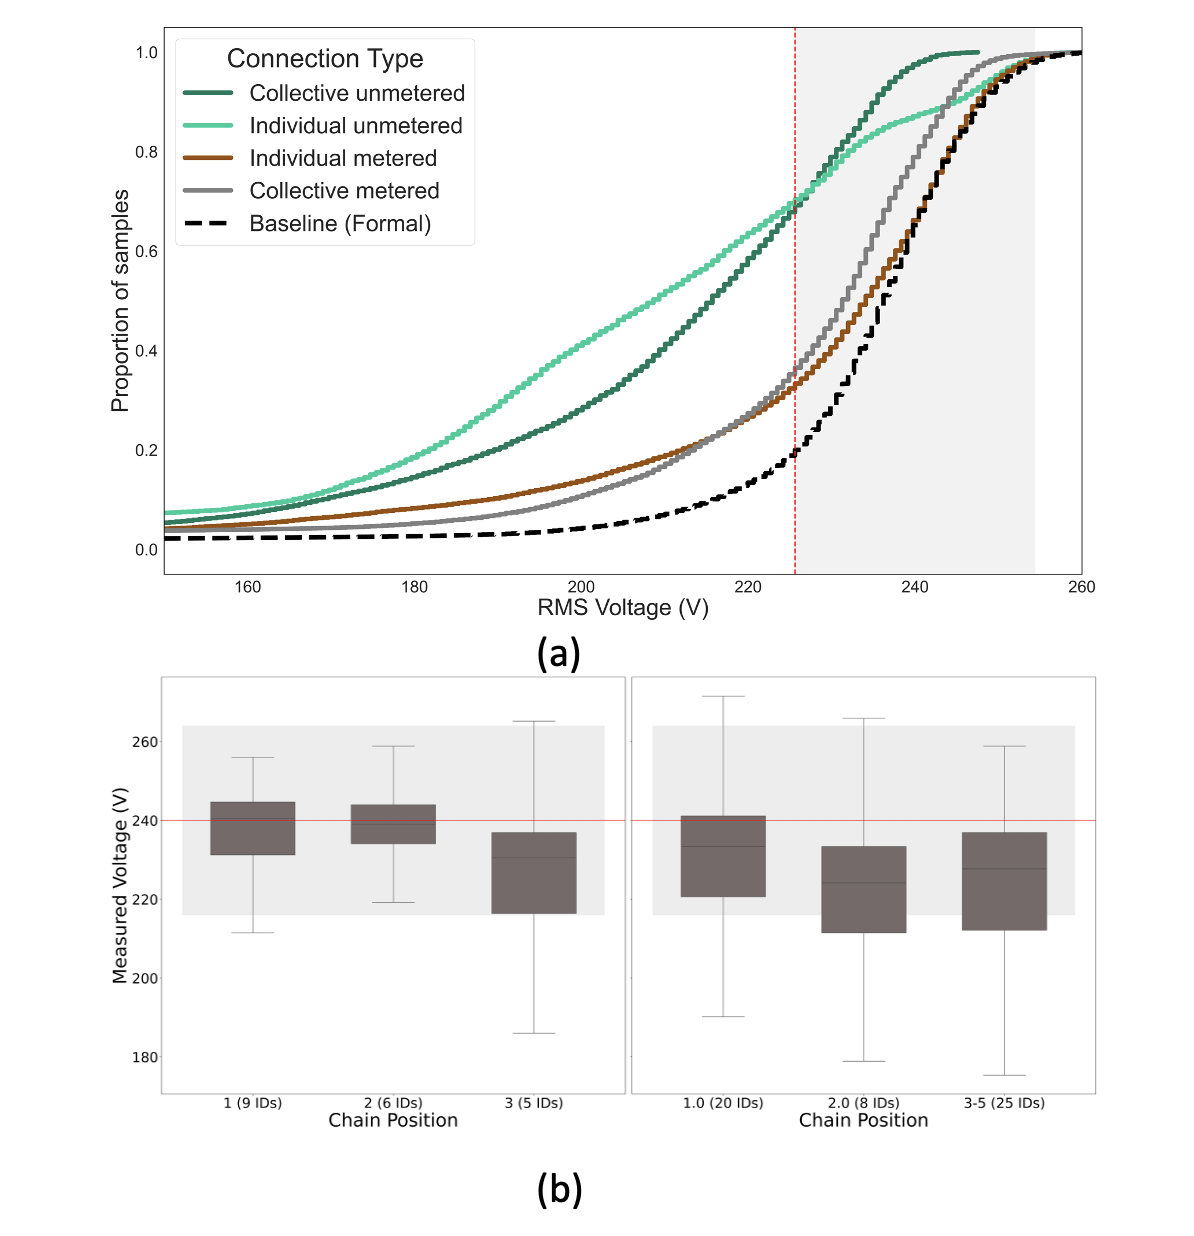
\includegraphics[width=0.9\linewidth]{figures/connections_chain_position.png} 
    \caption{Distribution of RMS voltage measurements by connection type and chain position. \textbf{(a)}: Empirical cumulative distribution functions (ECDF) compare voltage quality across different informal connection types and formal baseline. The vertical red line is the lower voltage limit of 225.6 V and the gray shaded area is the acceptable voltage range of 225.6–254.4V. \textbf{(b)}: Boxplots summarize voltage variations across chain positions, with the number of unique sensors (IDs) labeled per group. The red horizontal line is the nominal voltage of 240V.}
    \label{fig:cons_chain}
\end{figure}


\subsection{Timing and duration of poor voltage quality}

Voltage variations in informal settlements are particularly noticeable between 3:30-8pm and 5-10am as shown in Figure~\ref{fig:time_bracket_state}. This aligns with the inverse load curve, indicating that the voltage quality is poorer at times of day when homes and businesses need it the most. Our analysis further reveals that on average informal settlements experience approximately 6.3 hours undervoltage daily compared to 2.3 hours in the formal settlements. Figure~\ref{fig:v_tran_prob} shows the distribution of voltage interquartile range for each customer by time of day. We have a wider range of voltage values during peak than off-peak hours. We use this IQR as a measure of unpredictability. Figure~\ref{fig:time_bracket_state} shows the distribution of time spent in each voltage state. Informal settlements demonstrate longer dwell times in the low-voltage state and greater variability in each duration.
\begin{comment}
    Although most participants understood the pattern of these low voltage events and hours of the day with persistent low voltage events, it was challenging to plan daily activities because the voltage fluctuations were unpredictable. Voltage situations varied significantly from one hour to the next and from one day to the other, making it difficult for customers to know when voltage fluctuations and outages would occur. 
This made it difficult for users to adjust their activities around the erratic power supply. In situations where there were power outages, and appliances remained plugged in, power is often restored with momentary surges of high voltages that damage appliances. As one participant explained, “quote”. In situations where voltages were extremely low, certain appliances could not function properly. Electric kettles took longer to boil water and cooking coils took longer than expected to heat up, hence increasing the time required to prepare certain meals.
\end{comment}


\begin{figure}[H]
    \centering
    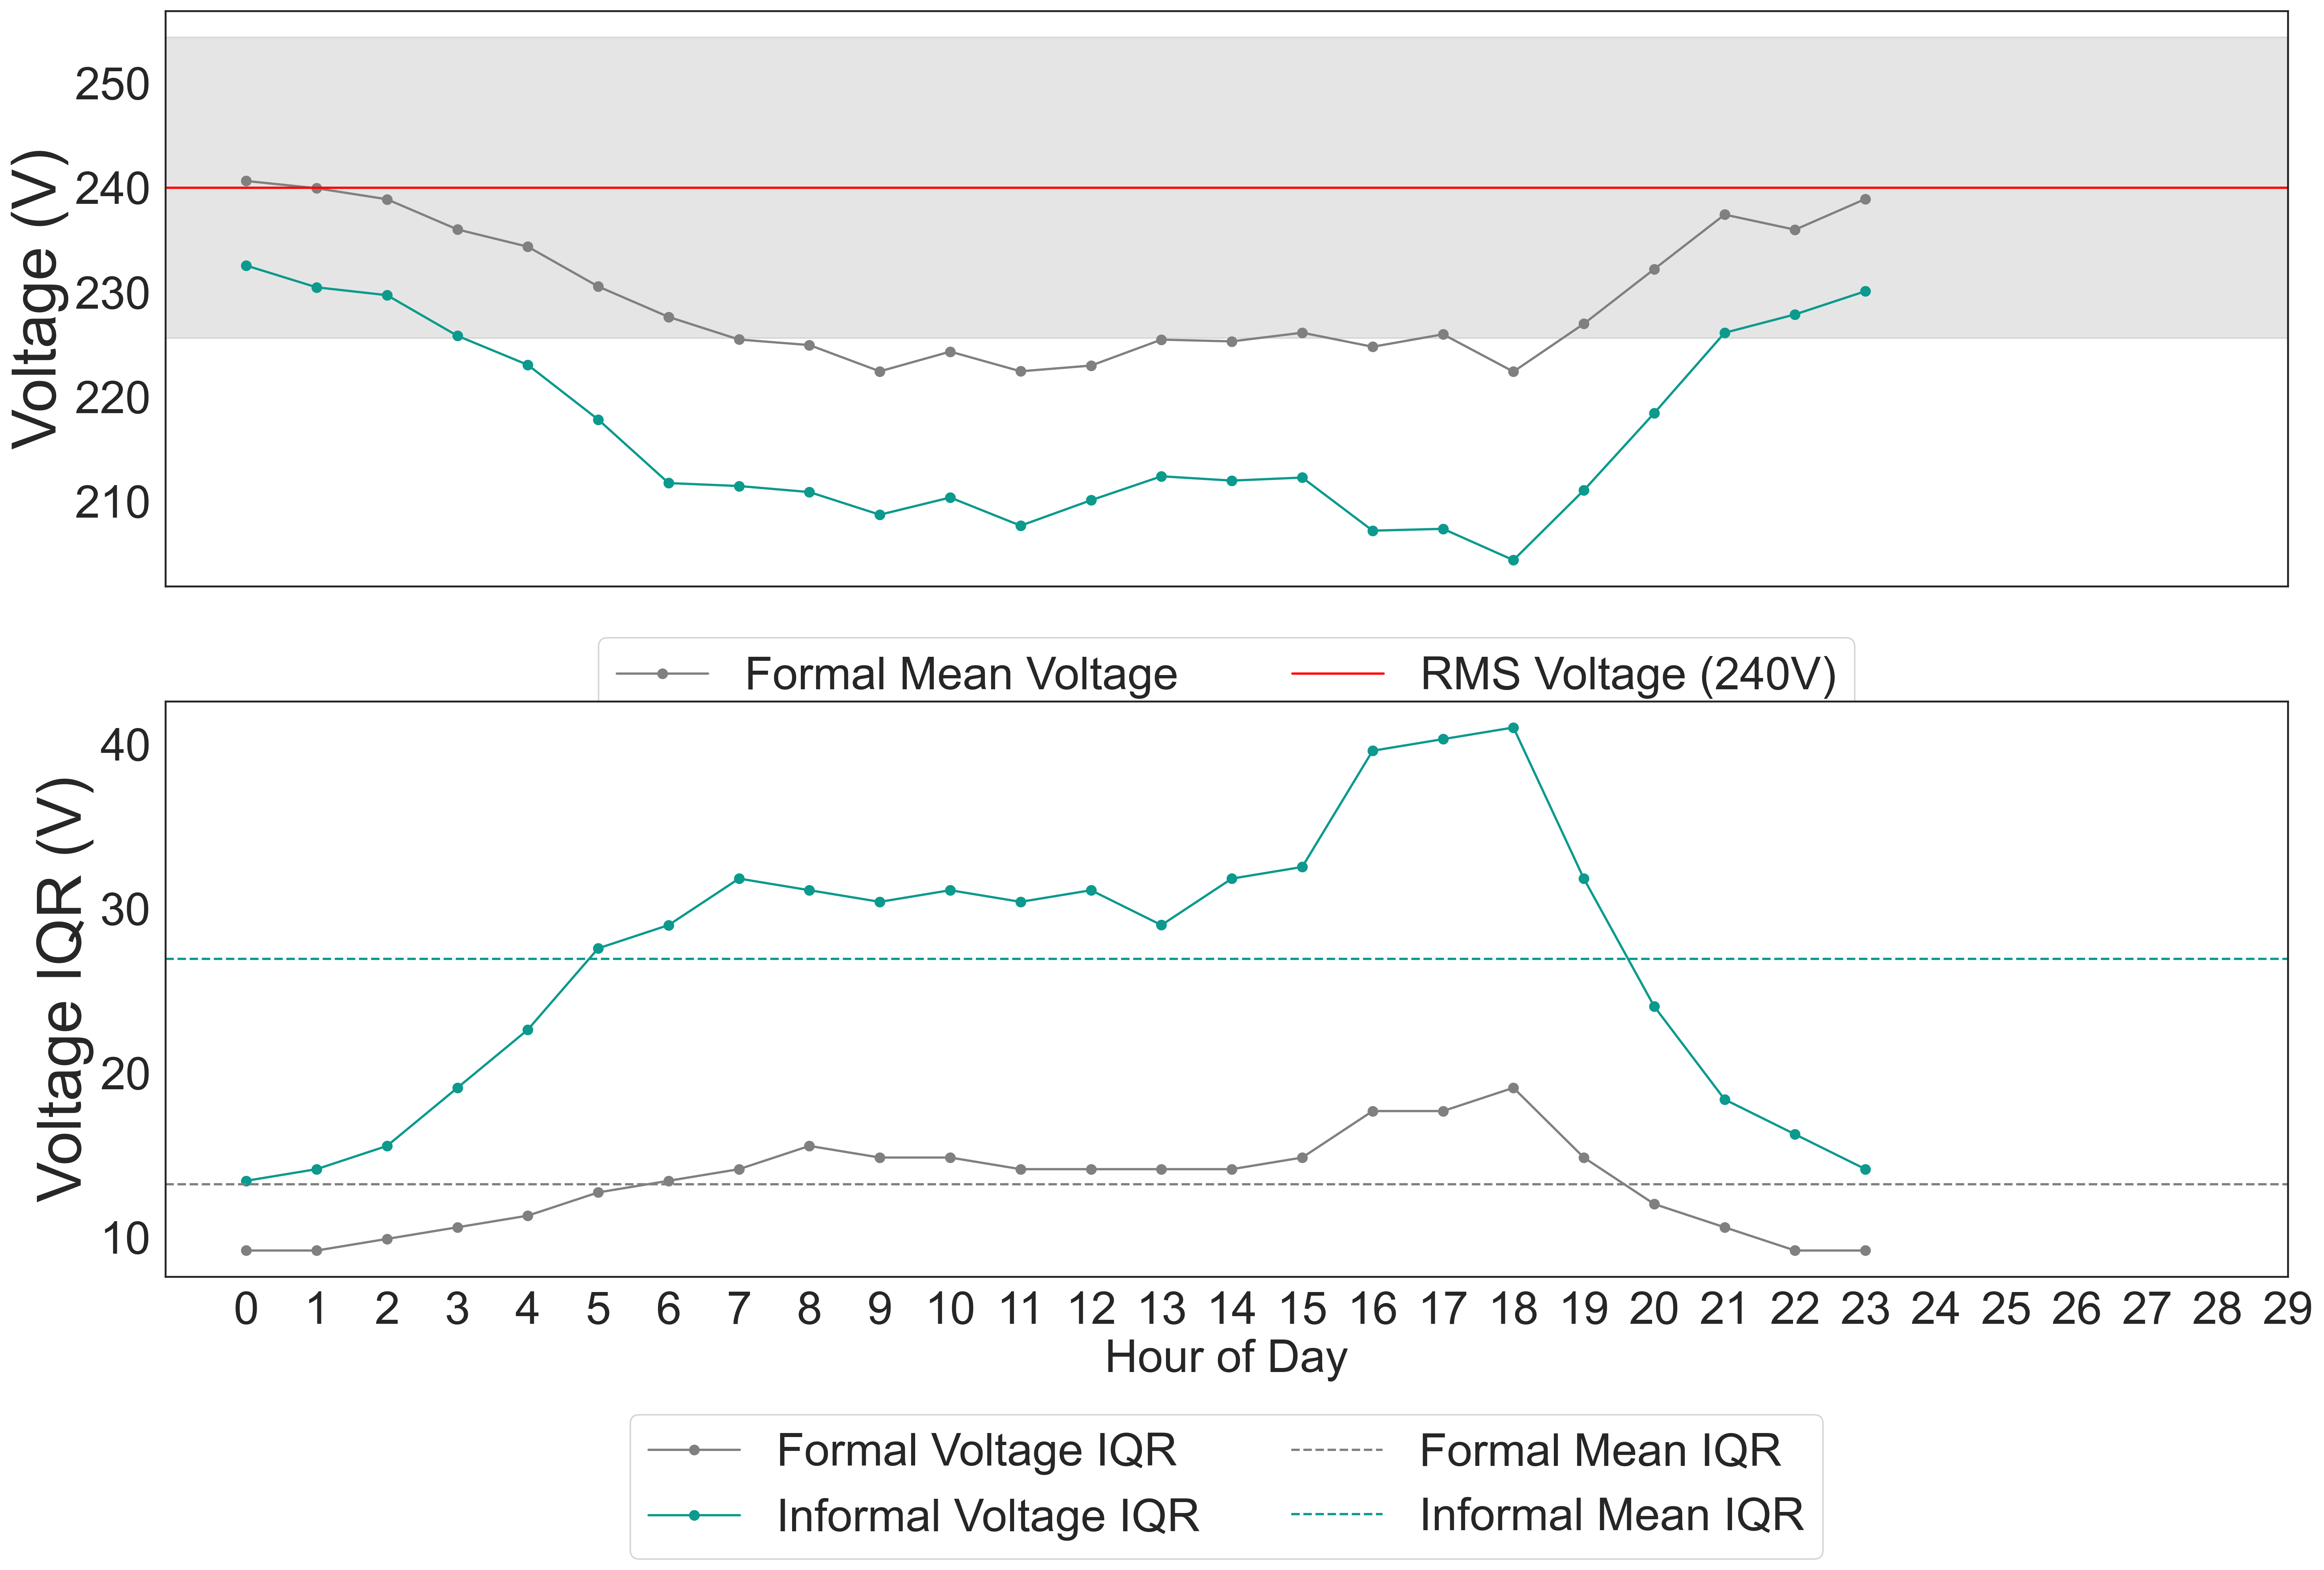
\includegraphics[width=0.9\linewidth]{figures/voltage_line_plot_hr.png} 
    \caption{Voltage distribution by time of day}
    \label{fig:v_tran_prob}
\end{figure}

\begin{figure}[H]
    \centering
    \includegraphics[width=0.95\textwidth]{figures/vol_state_duration.png}
    \caption{Distribution of duration in each voltage state by settlement type. This visualization highlights the persistence and timing of voltage conditions in informal settlements}
    \label{fig:time_bracket_state}
\end{figure}




\subsection{\suggestreplacesjl{Voltage State Transition Matrix and Entropy Analysis}{Markov Chain Voltage Quality Model and Entropy-Based Predictability Measures}}

\begin{comment}
    The heatmap in Figure~\ref{fig:markov} shows a log-normalized transition matrix of the Top 25 most frequent voltage state transitions. Due to the high dimensionality of the entire 108×108 matrix, we extracted the 25 most frequently observed states to form a compact, interpretable submatrix. Each state is defined by a triplet: Time-of-day (e.g., [18–20) hours), Duration class (how long the participant has remained in that state: 0–2, 2–4, or 4+ hours), and Voltage condition: Acceptable (A), Unacceptable (U), or Outage (O).
\end{comment}
The heatmap in Figure~\ref{fig:markov} shows a log-normalized transition matrix of the 25 most frequent voltage state transition probabilities based on the triplets defined in the methodology. \suggestreplacesjl{The dominant diagonal elements highlight temporal persistence in the voltage behavior, which is consistent with our semi-Markov assumptions. However, notable off-diagonal clusters reveal common transitions, such as shifts from Unacceptable to Outage states around evening hours (e.g., [18-20)) and sustained outages in certain time blocks.}{The dominant diagonal elements correspond to the system remaining in the same composite state within a given time-of-day bin. Structured off-diagonal entries---such as transitions to the next time-of-day bin with the same voltage condition and saturated duration class---also reflect voltage persistence; together, these entries confirm that voltage conditions tend to be temporally sticky, consistent with the duration-dependent dynamics captured by the enriched-state Markov model. However, notable off-diagonal clusters involving changes in the voltage condition itself reveal genuine state transitions, such as shifts from Unacceptable to Outage around evening hours (e.g., [18-20)) and sustained outages in certain time blocks. The prevalence of such entries indicates periods where voltage dynamics become less predictable.}

\begin{figure}[H]
    \centering
    \includegraphics[width=0.95\textwidth]{figures/markov_transition_matrix.png}
    \caption{Log-Normalized Transition Matrix of the Top 25 Most Frequent Voltage States.
Each state is defined by a triplet: Time-of-day (e.g., [18–20) hours), Duration class: (0–2, 2–4, or 4+ hours), and Voltage state: Acceptable (A), Unacceptable (U), or Outage (O).}
    \label{fig:markov}
\end{figure}

Figure ~\ref{fig:entropy_voltage} compares the entropy of voltage states and the probability of usable voltage across formal and informal settlements. \suggestreplacesjl{Entropy serves as a measure of unpredictability in voltage quality, where higher entropy values reflect greater variability in voltage behavior. Informal settlements tend to exhibit higher entropy levels, indicating more erratic voltage patterns, while formal areas generally show lower entropy and greater voltage stability.}{The conditional entropy $H(X_t \mid X_{t-1})$ quantifies the average per-row uncertainty of the transition matrix, weighted by the stationary distribution: when each composite state has few likely successors, the weighted average is low and the voltage process is predictable; when probability mass is dispersed across many successors---reflecting frequent, short-duration state changes and voltage condition shifts---the entropy is high. Informal settlements tend to exhibit higher entropy, indicating that their voltage dynamics are more erratic and harder to anticipate, while formal areas show lower entropy and more structured voltage behavior.} This pattern is further accompanied by the probability of usable voltage, with formal settlements consistently achieving higher probabilities of maintaining voltage within acceptable thresholds. Notably, sites such as kyeb, mlg2, and kbyo in informal settlements show both high entropy and low usable voltage probability, underscoring their vulnerability to poor and unpredictable power supply. These findings reinforce the connection between socioeconomic position (proxied by measuring informal against formal communities) infrastructure condition and voltage reliability, suggesting the need for targeted technical and policy interventions in informal areas.

\begin{figure}[H]
    \centering
    \includegraphics[width=0.95\textwidth]{figures/entropy_voltage_plot.png}
    \caption{\suggestreplacesjl{Comparison of entropy and usable voltage probability by site across informal and formal settlements. Entropy captures the predictability of voltage quality; higher entropy indicates more variability.}{Kiki: please specify which entropy measure is plotted here---the conditional entropy $H(X_t \mid X_{t-1})$ or the joint entropy $H(X_t, X_{t-1})$? The caption and surrounding body text should name the specific quantity. Whichever entropy definition is not used in any results figure or discussion should be removed from the Methodology section to avoid presenting unused formalism. If the plotted quantity is the conditional entropy, a suggested caption: ``Conditional entropy $H(X_t \mid X_{t-1})$ and probability of usable voltage by site, across formal and informal settlements. Higher conditional entropy indicates less predictable voltage dynamics.''}}
    \label{fig:entropy_voltage}
\end{figure}

{\color{sjlmutedblue}\textbf{[SJL20260306, Figure~\ref{fig:entropy_voltage} Note]}\ Kiki: the line segments connecting the dots on this plot appear to reuse the same red and green already assigned to the dot colors (informal vs.\ formal). Please recolor the line segments to a distinct color (e.g., gray or black) so they are visually differentiated from the dot markers, and add a legend entry or note defining what the line segments represent.}


\section{Discussion}

Our study reveals that electricity access in urban informal settlements cannot be meaningfully understood through the binary notion of access alone. By analyzing high-resolution voltage quality and reliability data from households and businesses in Kampala, we show that power quality, timing, wiring quality and infrastructural configuration are important dimensions of energy inequality and have significant implications for livelihoods, safety, and progress towards SDG 7.
Our findings show that 95\% of informal settlements are grid-connected but the quality of supply is severely compromised. Over 20\% of voltage samples in these areas fall below usable thresholds (Grade F), and households experience an average of 6.3 hours of undervoltage per day, nearly triple that of formal settlements. This highlights that being connected does not guarantee meaningful access, challenging metrics that define energy access solely in terms of connectivity and even more complex metrics that assess infrastructure presence.

Another major finding from our study is the clear performance gap in voltage quality between metered and unmetered users, even within the same informal settlements. Nearly 60\% of unmetered users’ voltage samples fell below the low voltage limit, compared to 20\% for metered users. This variation underscores the crucial role of behind-the-meter infrastructure in shaping electricity quality.

Beyond the severity of voltage drops, our findings reveal a pronounced temporal unpredictability in voltage quality, with the worst conditions occurring during peak usage hours between 5:00–10:00 am and 3:30–8:00 pm. These are the very hours when households are cooking, businesses are operating, and children are studying, making timing, not just quantity but a critical constraint. These unpredictable voltage fluctuation events often occur without advance warning or notice and makes it difficult for users to plan activities around it.

{\color{sjlmutedblue}\textbf{[SJL20260306, Note]}\ Kiki: the claims in the paragraph above---that voltage unpredictability concentrates during peak hours and that fluctuations are difficult to anticipate---are currently stated qualitatively. Can these be shown in a figure or quantified? For example, you could plot the conditional entropy (or the per-row entropy of the transition matrix) broken down by time-of-day bin to show that predictability degrades during the 5--10\,am and 3:30--8\,pm windows. Alternatively, a figure showing the variance or IQR of voltage by hour (you already have Figure~\ref{fig:v_tran_prob}) could be referenced here more explicitly to support this claim.}

These dynamics suggest a form of temporal energy poverty, a condition in which electricity is technically available and may even satisfy minimum tier requirements, yet remains unreliable or unusable at the times when it is most needed. While the Multi-Tier Framework (MTF) has significantly advanced electricity access measurement by moving beyond binary connection metrics to incorporate dimensions such as capacity, reliability, and voltage adequacy, our findings indicate that temporal persistence and predictability remain insufficiently captured. Households may meet formal tier thresholds while still experiencing prolonged or unpredictable voltage deviations that disrupt daily routines. Cooking, refrigeration, and income-generating activities are particularly sensitive to such variability; when voltage quality fluctuates unpredictably, it can lead to spoiled goods, reduced productivity, equipment stress, and lost time, especially for informal businesses that rely on basic electrical appliances. These results suggest that temporal stability, not merely compliance with static thresholds, is central to defining functional electricity access.

\begin{comment}
    These dynamics suggest a form of "temporal energy poverty", a condition where energy is technically present but not usable when most needed. While energy access is typically measured in binary terms (connected or not), our findings argue for a more nuanced view that includes availability, predictability, and temporal alignment with daily needs. For example, cooking or refrigeration routines disrupted by unpredictable voltage quality result in lost time, spoiled goods, and appliance malfunction, particularly for informal businesses that rely on basic electrical tools or appliances.
\end{comment}

Our findings also underscore the importance of temporal modeling in understanding electricity reliability. A purely instantaneous classification would obscure the fact that users often experience long spells of poor voltage quality, which may be more damaging than brief, fluctuating voltages. \suggestreplacesjl{The semi-Markov structure helps capture this “stickiness” in Unacceptable states.}{By encoding duration class in the state definition, the Markov model captures this ``stickiness'' in Unacceptable states: a household that has persisted in a given voltage condition for a longer period exhibits distinct transition probabilities from one that just entered.}

{\color{sjlmutedblue}\textbf{[SJL20260305, Suggested New Text]}\ The entropy analysis makes this concrete: in settlements where voltage conditions change frequently and unpredictably, each row of the transition matrix has probability dispersed across many successor states, yielding higher conditional entropy. For households, this translates directly into an inability to plan cooking, business, or study activities around the power supply---not because power is always poor, but because its quality at any given moment is difficult to anticipate from its recent history.}

Together, these findings suggest that electricity access frameworks must evolve to better capture the temporal and infrastructural dimensions of service quality, particularly in rapidly urbanizing informal contexts. While the Multi-Tier Framework has advanced access measurement beyond binary connection indicators, our results demonstrate that persistence, volatility, and predictability of voltage conditions remain underexamined components of functional electrification. Policy efforts should therefore extend beyond grid expansion and nominal tier compliance to incorporate high-resolution power quality monitoring, infrastructure equity at the household level, and targeted investments in safe and appropriately sized service connections. Integrating temporal voltage metrics into national reporting systems and SDG 7 monitoring could improve alignment between measured access and lived experience. In parallel, utilities and planners should consider community-based monitoring, proactive load and power quality forecasting, and real-time communication tools to mitigate the impacts of voltage instability. Without such measures, households in informal settlements may remain formally connected and statistically “served,” yet functionally constrained in their ability to use electricity for productive, health-supporting, and welfare-enhancing activities.


%Although electrification rates in urban Uganda are high, our findings show that voltage conditions in informal settlements undermine the actual usability of electricity, challenging traditional metrics of energy access. Households and businesses in informal settlements experience persistent undervoltage and erratic fluctuations, reflecting deeper structural inequities in grid planning and service delivery. These deficiencies not only compromise daily appliance use and livelihoods but also obstruct broader energy transition goals such as electrification of productive uses and equitable decarbonization. Addressing power quality thus becomes essential to ensuring that electrification truly enables social and economic inclusion.

%Connection modalities are not only technical configurations but reflect systemic inequalities in access, affordability, and infrastructure investment. In our analysis, unmetered users face more severe and sustained undervoltage conditions than metered ones, with informal or shared connections exhibiting greater instability. These results point to the role of sub-distribution infrastructure, such as wiring quality and connection types as a critical determinant of power quality. Without attention to these last-mile issues, grid expansion efforts may fail to deliver reliable electricity, particularly for vulnerable populations living in informal or underserved urban areas.

%Voltage fluctuations were most severe during peak hours—morning and evening—when electricity demand is high. In informal settlements, these fluctuations were not only larger in magnitude but also more unpredictable, as shown by entropy analysis. This unpredictability makes planning difficult for users and suggests a mismatch between infrastructure capacity and load growth. Our deployment of real-time, outlet-level sensors reveals how granular sensing can surface such dynamics, offering a scalable pathway for utilities to monitor and improve low-voltage networks.

%Poor power quality and reliability (PQR) remain critical barriers to meaningful electrification, especially for high-power loads such as electric cooking and transportation. Most modern e-cooking appliances cannot operate under extreme low voltages and are at risk of damage from frequent fluctuations and outages. PQR issues are not limited to transmission bottlenecks—they are prevalent at the supply and distribution tiers, directly affecting households and small businesses, and by extension, livelihoods. Addressing voltage quality is thus fundamental for unlocking the full socioeconomic potential of electrification. Furthermore, there is an urgent need for improved methods to measure PQR at scale and for a deeper understanding of its spatial and temporal impacts. Without addressing voltage reliability, urban electrification cannot meaningfully support decarbonization, livelihood enhancement, or broader energy transition goals.

%These findings underscore the importance of temporal modeling in understanding electricity reliability. A purely instantaneous classification would obscure the fact that users often experience long spells of poor power quality, which may be more damaging than brief, fluctuating outages. The semi-Markov structure helps capture this “stickiness” in Unacceptable states.

%Building on the insights from this study, future work will explore the sensitivity of electric cooking (e-cooking) appliances to poor voltage quality. Many modern e-cooking devices require consistent voltage supply and may underperform or become damaged under low or highly fluctuating voltages—conditions frequently observed in our dataset. We also aim to assess the impact of widespread e-cooking adoption on grid infrastructure, particularly in already stressed distribution systems. Understanding these interactions will help inform infrastructure planning, appliance design standards, and energy access programs that seek to promote clean cooking while preserving grid reliability.

%Enforce minimum wiring standards and connection modalities to improve quality 
%Formalize the unlicensed wire men who are connecting households to the grid illegally 
%Poor voltage quality limits the benefits of electrification efforts and promote economic exclusion. The damaged appliances resulting from poor voltage quality limits productivity at the household and business level. 
%Invest in smart grid sensing technologies that currently available to track and measure voltage quality.  
%Acknowledge voltage quality as an issue that hampers economic growth and impacts the financial value of electricity infrastructure investments

\section{Conclusion}

This study provides new evidence on the quality and reliability of electricity access in urban informal settlements, using high-frequency sensor data from households and businesses in Kampala. Our findings show that while connectivity rates are high, power quality is often severely compromised — particularly for unmetered users and during peak usage hours. These conditions undermine the functionality of basic appliances, disrupt daily routines, and limit the ability of households and enterprises to benefit from electricity access.

The results highlight the need to move beyond binary definitions of energy access and adopt a multidimensional framework that includes power quality, temporal reliability, and behind-the-meter infrastructure. Addressing these challenges will require targeted investments in low-cost, safe wiring, improved regulatory pathways for connection formalization, and monitoring tools that make power quality visible to both utilities and end-users.

While the study is focused on Kampala and limited to two months of monitoring, the patterns observed reflect broader challenges in rapidly urbanizing contexts across sub-Saharan Africa. Future work could explore appliance-level impacts, expand monitoring to different seasons, and assess the effectiveness of community-based interventions aimed at improving voltage stability and user awareness.


\textbf{Declaration of generative AI and AI-assisted technologies in the manuscript preparation process}

During the preparation of this manuscript, the author(s) used ChatGPT to check grammar and refine certain sentences. After using this tool/service, the author(s) reviewed and edited the content as needed and take(s) full responsibility for the content of the published article.

\bibliographystyle{elsarticle-num} 
\bibliography{references} %% Use references.bib file

\end{document}






